Disagreements between the obtained and the \emph{aRTist} simulated projections can be found by subtracting one projection from the other. Any values too big in magnitude can be considered as a defect. However, in the previous chapters, it was found that x-ray photons behave randomly and differences in the comparison can be due to chance. Thus, the comparisons should be done in the face of uncertainty.

A pixel by pixel hypothesis test was proposed to do defect detection. To illustrate this method of inference, the projections from the dataset \texttt{AbsFilter} at \ang{120} was used. To recap, 20 replicate projections of a test sample, with purposefully manufactured voids, were obtained. \emph{aRTist} was used to create a simulation of that projection but as if the voids were not there. Thus, the method should pick these voids up.

Beforehand, linear shading correction was applied to the projections. The \emph{aRTist} projections were shading corrected using the simulated greyscale projections. The 20 replicate projections were split into two. 19 randomly selected projections were used for the variance-mean model to fit onto. The remaining projection was compared with the \emph{aRTist} projection. This remaining projection and the \emph{aRTist} projections are shown in Figures \ref{fig:inference_inferenceIntro_inference_scan} and \ref{fig:inference_inferenceIntro_inference_artist} respectively.

A gamma GLM, with a basic linear relationship, was used for the variance-mean model, as described in Chapter \ref{chapter4}. The variance was predicted using the grey value in the \emph{aRTist} simulation as the predictor variable.

The test statistic, for the pixel located at $(x,y)$, is
\begin{equation}
  Z_{x,y} =
  \dfrac{
    \text{projection}_{x,y} - \emph{aRTist}_{x,y}
  }
  {
    \sqrt{s^2\left[\emph{aRTist}_{x,y}\right]}
  }
\end{equation}
where $s^2\left[\emph{aRTist}_{x,y}\right]$ is the predicted grey value variance. The test statistic was calculated for each pixel in the ROI, that is, pixels which represent the test sample. The ROI was created by manually segmenting the test sample from the projection.

It is important to identity which quantites are random and which are not. For high photon rates, it was shown in the previous chapters that the grey values in the projection can be modelled using a Normal distribution. Thus, $\text{projection}_{x,y}$ is a random quantity. The simulation $\emph{aRTist}_{x,y}$ is not random because this was obtained through a computer software. Given the 19 selected projections used for training the variance-mean model, the variance prediction $s^2\left[\emph{aRTist}_{x,y}\right]$ is not random because the variance-mean model was fitted before encountering the remaining projection to be compared with \emph{aRTist}. The variance-mean model can be made random if a different set of 19 projections was used to train the model each time this inference was conducted, but this shall not be considered here.

If there are no significant differences between the obtained and \emph{aRTist} projections, then the randomness of the test statistics can be approximately quantified as
\begin{equation}
Z_{x,y}\sim \normal(0,1) \ .
\end{equation}
As with usual statistical convention, an upper case $Z$ denotes a random variable. A lower case $z$ denotes a realisation or an observation of that random variable.

For each pixel, a test statistic was calculated, which forms a $z$ image. A test statistic too large in magnitude, relative to the anticipated variance, will classify that pixel as a positive result. In two-tailed hypothesis testing \citep{pearson1900on, neyman1933on, fisher1970statistical}, $p$-values can be used to represent the test statistics in a different way
\begin{equation}
  p_{x,y} = 2(1-\Phi(|z_{x,y}|))
\end{equation}
which can takes values $0\leqslant p_{x,y} \leqslant 1$. A $p$-value too small is considered a positive result. The $p$-values are shown in Figure \ref{fig:inference_inferenceIntro_inference_pvalue}.

\begin{figure}
  \centering
  \centerline{
    \begin{subfigure}[b]{\subSize}
      \includegraphics[width=\textwidth]{../figures/inference/inferenceIntro_scan.eps}
      \caption{Obtained projection (\SI{}{\adu})}
      \label{fig:inference_inferenceIntro_inference_scan}
    \end{subfigure}
    \begin{subfigure}[b]{\subSize}
      \includegraphics[width=\textwidth]{../figures/inference/inferenceIntro_artist.eps}
      \caption{\emph{aRTist} projection (\SI{}{\adu})}
      \label{fig:inference_inferenceIntro_inference_artist}
    \end{subfigure}
  }
  \centerline{
    \begin{subfigure}[b]{\subSize}
      \includegraphics[width=\textwidth]{../figures/inference/inferenceIntro_logp.eps}
      \caption{$-\log p\text{-values}$}
      \label{fig:inference_inferenceIntro_inference_pvalue}
    \end{subfigure}
    \begin{subfigure}[b]{\subSize}
      \includegraphics[width=\textwidth]{../figures/inference/inferenceIntro_positivePixels.eps}
      \caption{Positive pixels overlaid on a)}
      \label{fig:inference_inferenceIntro_inference_positivePixels}
    \end{subfigure}
  }
  \caption{The obtained projection of the test sample (a), from the \texttt{AbsFilter} at \ang{120} dataset, was compared to the \emph{aRTist} projection (b) to detect purposefully manufactured voids. The $p$-values (c) obtained were used for hypotheses testing. Pixels detected as positive are shown in red in d) using the \cite{benjamini1995controlling} procedure at the 5\% false discovery rate level.}
  \label{fig:inference_inferenceIntro_inference}
\end{figure}

The resulting $p$-values are concerning. This is because the $p$-values are not very smooth on the surfaces of the sample. It should be expected that small $p$-values are in areas of the defects. Pixels were tested positive or considered to be evidence of a defect, when $|z_{x,y}|>\inputNumber{../figures/inference/inferenceIntro_critical.txt}$ to 2 decimal places. This value was chosen by controlling the false discovery rate at 5\% using the \cite{benjamini1995controlling} (BH) procedure. The positive pixels are shown in Figure \ref{fig:inference_inferenceIntro_inference_positivePixels}.

This proposed method for defect detection failed because too many false positives were detected. These false positives appeared to have some structure, for example, clustering in the corners or on surfaces. Also, false negatives were detected because not all of the defects were detected.

Model misspecification appeared to be the main source of error. The test statistics and $p$-values were inspected in Figure \ref{fig:inference_inferenceIntro_histogram}. It can be seen that the test statistics were not compatible with the standard Normal distribution. Also, the majority of the $p$-values did not look uniformly distributed. This seems to suggest that the assumption of $Z_{x,y}\sim \normal(0,1)$ is incorrect.

\begin{figure}
  \centering
  \centerline{
  \begin{subfigure}[b]{\subSize}
    \includegraphics[width=\textwidth]{../figures/inference/inferenceIntro_histogram.eps}
    \caption{Histogram}
  \end{subfigure}
  \begin{subfigure}[b]{\subSize}
    \includegraphics[width=\textwidth]{../figures/inference/inferenceIntro_pValue.eps}
    \caption{$p$-values}
    \label{fig:inference_inferenceIntro_pvalue}
  \end{subfigure}
}
  \caption{a) The histogram of the test statistics, from the \texttt{AbsFilter} projection at \ang{120}, is compared with the standard Normal distribution. The standard Normal distribution is known as the null distribution in this scenario. b) The $p$-values are ordered and plotted. The critical region corresponds to controlling the false discovery rate at the 5\% level using the \cite{benjamini1995controlling} procedure. The dotted line shows the result if the $p$-values were uniformly distributed.}
  \label{fig:inference_inferenceIntro_histogram}
\end{figure}

This chapter recaps hypothesis testing, for a single test and then for multiple tests, treating each pixel as a test. Assumptions used in the hypotheses testing can be relaxed by using the empirical null \citep{efron2004large}, which is reviewed here. The empirical null is then extended to an image filter, called the empirical null filter. This filter adjusts each test statistic according to its neighbours, ironing out false positive results. Simulations and results are shown towards the end of the chapter.

\section{Literature Review}

Consider a test statistic $Z$ from a pixel. If there are no defects, then the statistic is null and has the null distribution $Z|H_0\sim\normal(0,1)$. This can be described by specifying the random variable as $Z\sim\normal(\mu,1)$ and the null hypothesis as $H_0:\mu=0$. A hypothesis test can judge how much $Z$ deviates from 0 by defining the alternative hypothesis $H_1:\mu\neq 0$. A statistic which does not has the null distribution is known as non-null.

In two-tailed hypothesis testing \citep{pearson1900on, neyman1933on, fisher1970statistical}, the $p$-value can be compared with the user-defined size of the test $\alpha$, also known as the significance level in this specific example. A positive result is declared when $p<\alpha$, else it is a negative result. Correct and incorrect testing of the statistics can occur. For example, testing a null statistic as positive is known as a false positive. It can be shown that $\alpha$ controls the false positive rate. $\alpha=5.0\%$ is a typical choice \citep{wasserstein2019moving} and is used throughout this thesis.

Multiple hypotheses testing occurs when there are more than one hypotheses to test. For example, $N$ pixels can be tested where the test statistics are $Z_1, Z_2, \dotsc, Z_N$ and $Z_i\sim\normal(\mu_i,1)$ for $i=1,2,\dotsc,N$. The null hypotheses are $H_{0,i}:\mu_i=0$ and are tested against the alternative $H_{1,i}:\mu_i\neq 0$ for $i=1,2,\dotsc,N$. Let the corresponding $p$-values be $p_1, p_2, \dotsc, p_N$.

The uncorrected test classify any $p_i<\alpha$ as positive. This is flawed because the possibility of obtaining at least one false positive increases as the number of tests increases \citep{shaffer1995multiple}. This method does control the per-comparison error rate (PCER) \citep{benjamini1995controlling}. PCER is the proportion of false positives out of all tests. The notation for the number of true/false positive/negatives obtained are defined in Table \ref{table:inference_randomvariables}. Using the notation, the PCER is defined as
\begin{equation}
  \text{PCER}=
  \dfrac{1}{N}
  \expectation[V]
  \ .
\end{equation}
It can be seen that if the uncorrected test controls the false positive rate such that $\expectation[V]/N_0 = \alpha$, then it controls the PCER such that
\begin{equation}
  \text{PCER}\leqslant\alpha \ .
\end{equation}

\begin{table}
  \centering
  \begin{tabular}{l|cc|c}
    &Negative&Positive&Total\\\hline
    Null & $U$ & $V$ & $N_0$\\
    Non-null & $T$ & $S$ & $N-N_0$\\\hline
    &$N-R$&$R$&$N$
  \end{tabular}
  \caption{Random variable definitions for the number of true/false positives/negatives made in multiple hypotheses testing}
  \label{table:inference_randomvariables}
\end{table}

The Bonferroni correction \citep{shaffer1995multiple, bland1995multiple, perneger1998what} controls the family-wise error rate (FWER) \citep{shaffer1995multiple} where
\begin{equation}
  \text{FWER} = \prob(V\geqslant1) \ .
  \label{eq:inference_fwer}
\end{equation}
This is done by adjusting the size of the test to be $\alpha/N$. By using the adjusted size, then $\text{FWER}=1-\left[(1-\alpha/N)^N\right]$. Using the approximation $(1-\alpha/N)^N\approx 1-\alpha$ then $\text{FWER}\approx \alpha$. This shows that the Bonferroni correction controls the family-wise error rate such that
\begin{equation}
  \text{FWER} \leqslant \alpha \ .
\end{equation}
In practice, the Bonferroni correction is not very powerful \citep{perneger1998what}, meaning it gives too many false negatives. This is because the correction traded too many false positives for false negatives.

The \cite{benjamini1995controlling} (BH) procedure controls the false discovery rate (FDR) \citep{benjamini2010discovering} rather than the PCER or FWER. The FDR is the proportion of false positives out of all positive results, that is
\begin{equation}
  \text{FDR} = \expectation\left[\dfrac{V}{R}\right]
  \ .
\end{equation}
It is defined that $V/R=0$ when $R=0$.

The BH procedure adjusts the size of the test between the Bonferroni correction and the uncorrected test. It adapts to the data and chooses different sizes for different data. The procedure is as follows, the $p$-values are ordered such that $p_{(1)}\leqslant p_{(2)}\leqslant \dotsc \leqslant p_{(N)}$. Suppose a size $\alpha$ is provided beforehand. The size is adjusted to
\begin{equation}
  \alpha_{\text{BH}} = \frac{\alpha k}{N}
\end{equation}
where
\begin{equation}
  k\text{ is the largest }i\text{ for which }p_{(i)}\leqslant\frac{i}{N}\alpha
  \ .
\end{equation}
This test the statistics with $p$-values $p_{(1)},p_{(2)},\dotsc,p_{(k)}$ as positive. For the case where $p_{(1)}>\alpha/N$ then $k=1$ so that the Bonferroni correction is used when there are no positive results, this is only for illustration purposes. For example in Figure \ref{fig:inference_inferenceIntro_pvalue}, the $p$-values were plotted against their order so that the critical boundary was shown by a linear curve with gradient $\alpha/N$.

The BH procedure comes from the fact that if all the statistics are null and independent, then the $p$-values are uniformly distributed \citep{simes1986improved}. However, it can be shown that the BH procedure works for many scenarios of dependencies \citep{benjamini2001control}. It can be shown that the BH procedure controls the FDR such that
\begin{equation}
  \text{FDR}\leqslant\alpha
\end{equation}
\citep{benjamini1995controlling}.

In summary, the uncorrected, Bonferroni and BH correction controls for different error rates according to the threshold $\alpha$, summarised in Table \ref{table:inference_corrections}.

\begin{table}
    \centering
    \begin{tabular}{l|l}
        Correction&Controls for\\\hline
        No correction&$\text{PCER}\leqslant\alpha$\\
        Bonferroni&$\text{FWER}\leqslant\alpha$\\
        BH&$\text{FDR}\leqslant\alpha$
    \end{tabular}
    \caption{Different types of corrections for multiple hypotheses testing are listed here, along with what they control for.}
    \label{table:inference_corrections}
\end{table}

Consider a small example where a $\SI{200}{\pixel}\times\SI{200}{\pixel}$ section of the $z$ image was investigated, as shown Figure \ref{fig:inference_inferenceSubsample1_histogram}. The distribution of the test statistics appeared Normal but not centred at zero. By using the BH procedure to obtain a critical region of $|Z|>\input{../figures/inference/inferenceSubsample1_criticalBoundary.txt}$ to 2 decimal places, almost half of the pixels were tested positive at the 5\% FDR level. It is questionable whether such many positive results are sensible, in particular, in an area where defects were not expected.

\begin{figure}
  \centering
    \centerline{
    \begin{subfigure}[b]{\subSize}
      \includegraphics[width=\textwidth]{../figures/inference/inferenceSubsample1_zImage.eps}
      \caption{Test statistics}
    \end{subfigure}
    \begin{subfigure}[b]{\subSize}
      \includegraphics[width=\textwidth]{../figures/inference/inferenceSubsample1_histogram.eps}
      \caption{Histogram}
    \end{subfigure}
    }
    \caption{The resulting test statistics for the \texttt{AbsFilter} projection at \ang{120} are shown in a). A $\SI{200}{\pixel}\times\SI{200}{\pixel}$ sub-image was taken shown by the dashed lines. A histogram of the test statistics in the sub-image is shown in b). The critical region corresponds to the 5\% FDR level.}
    \label{fig:inference_inferenceSubsample1_histogram}
\end{figure}

This problem commonly occurs in large scale multiple hypotheses testing \citep{efron2004large} such as in microarrays \citep{hedenfalk2001gene, efron2002empirical, efron2003robbins}. It appeared that the null distribution was misspecified as $Z_i|H_{0,i}\sim\normal(0,1)$ when in reality they are distributed as $Z_i|H_{0,i}\sim\normal(\mu_0,\sigma_0^2)$, where $\mu_0$ and $\sigma_0$ are the null mean and null standard deviation respectively.

In practice, $\mu_0$ and $\sigma_0$ are unknown. The empirical null \citep{efron2004large} replaces the parameters of the null distribution with its estimate. Suppose $\widehat{\mu}_0$ and $\widehat{\sigma}_0$ are the estimated null mean and null standard deviation respectively. The statistics are specified by $Z_i\sim\normal(\mu_i, \widehat{\sigma}_0^2)$ so that the following null hypotheses $H_{0,i}:\mu_i=\widehat{\mu}_0$ are tested against $H_{1,i}:\mu_i\neq\widehat{\mu}_0$ for $i=1,2,\dotsc,N$.

In \cite{efron2004large}, a few assumptions were made in order to obtain the estimators $\widehat{\mu}_0$ and $\widehat{\sigma}_0$. Let the test statistic $Z$ have the p.d.f.
\begin{equation}
  p_Z(z) =
  \pi_0 p_{Z|H_0}(z) + \pi_1 p_{Z|H_1}(z)
\end{equation}
where $0\leqslant\pi_0\leqslant 1$ and  $\pi_1 = 1-\pi_0$. In addition, the null distribution is
\begin{equation}
  p_{Z|H_0}(z) =
  \dfrac{1}{\sqrt{2\pi}\sigma_0}
  \exp\left[
    -\dfrac{1}{2}
    \left(
      \dfrac{z-{\mu}_0}{\sigma_0}
    \right)^2
  \right]
\end{equation}
as it was assumed to be Normal. The non-null distribution $p_{Z|H_1}(z)$ does not need to be specified. Assume that the majority of the data are null and non-null test statistics are rare, say $\pi_0>0.9$ \citep{efron2004large}, then around the mode, the probability density function would be dominated by the null distribution. This implies that
\begin{equation}
  p_{Z}(z) \approx \pi_0 p_{Z|H_0}(z)
\end{equation}
for values of $z$ around the mode. Finding the mode for $p_{Z}(z)$ and $p_{Z|H_0}(z)$ should yield the same solution. This justify the use of the mode for the empirical null mean \citep{efron2004large}
\begin{equation}
  \widehat{\mu}_0 = \argmax\widehat{p}_Z(z)
\end{equation}
where $\widehat{p}_Z(z)$ is the density estimation of $p_Z(z)$, for example it could be a smoothing spline fitted onto the histogram \citep{efron2004large}.

The null standard deviation is estimated from the log density \citep{efron2004large}. For values of $z$ at and around the mode
\begin{equation}
  \ln p_{Z}(z) =
  \ln\left[
    \dfrac{\pi_0}{\sqrt{2\pi}{\sigma}_0}
  \right]
  -\dfrac{1}{2}
  \left(
    \dfrac{z-{\mu}_0}{{\sigma}_0}
  \right)^2
  \ .
\end{equation}
Taking derivatives
\begin{align}
  \dfrac{\partial}{\partial z} \ln p_{Z}(z) &=
  -\left(
    \dfrac{
      z-{\mu}_0
    }
    {
      {\sigma}_0^2
    }
  \right)
  \\
  \dfrac{\partial^2}{\partial z^2} \ln p_{Z}(z) &=
  -\dfrac{
    1
  }
  {
    {\sigma}_0^2
  }
\end{align}
which motivates the estimator \citep{efron2004large}
\begin{equation}
  \widehat{\sigma}_0 = \left[
    \left.
      -\dfrac{\partial^2}{\partial z^2}\ln\widehat{p}(z)
    \right|_{z=\widehat{\mu}_0}
  \right]^{-1/2}
  \ .
  \label{eq:inference_nullStdEstimator}
\end{equation}
The evaluation of $z=\widehat{\mu}_0$ is used because at the mode, it was assumed that the null test statistics would dominate and non-null test statistics would not contribute much to the density estimate.

This method does not need estimations of $\pi_0$ which makes it quite convenient. Estimations of $\pi_0$ are discussed in literature such as \cite{benjamini2000adaptive, pounds2003estimating, storey2003statistical, pounds2004improving, langaas2005estimating, durnez2014posthoc}. \cite{efron2004large} motivated the use of the empirical null by investigating various types of false discovery rates \citep{storey2002direct, storey2003positive, efron2002empirical, efron2007size} which will not be discussed here.

The empirical null is used widely, including in neuroimaging \citep{schwartzman2008false, schwartzman2009empirical} and has been extended to include non-Normal null distributions \citep{schwartzman2008false, schwartzman2008empirical}. There exist various methods for the empirical null, for example, \cite{schwartzman2008empirical} used Poisson regression on the histogram counts in regions where the null statistics dominate. The empirical characteristic function was used in \cite{jin2007estimating}.

\section{Empirical Null}

Returning to the sub-image example in Figure \ref{fig:inference_inferenceSubsample1_histogram}. The histogram was smoothed using a kernel density estimate \citep{parzen1962on, friedman2001elements} as shown in Figure \ref{fig:inference_inferenceSubsample1_densityEstimate}. The kernel density estimate \citep{parzen1962on} is
\begin{equation}
  \widehat{p}_Z(z)=
  \frac{1}{nh}
  \sum_{i=1}^n\phi\left(
    \dfrac{z_i-z}{h}
  \right)
  \label{eq:inference_kernel_density_estimate}
\end{equation}
where $h$ is the bandwidth, $\phi(x)$ is the standard Normal density and $n=N$ is number of terms in the summation. The bandwidth was chosen such that
\begin{equation}
  h = (0.9n^{-1/5}\ + 0.16) \times \text{min}\left(s_z,\text{IQR}_z/1.34\right)
  \label{eq:inference_ourruleofthumb}
\end{equation}
where $s_z$ and $\text{IQR}_z$ are the sample standard deviation and sample interquartile range. This bandwidth is justified later on in this section.

\begin{figure}
  \centering
  \includegraphics[width=\subSize]{../figures/inference/inferenceSubsample1_densityEstimate.eps}
  \caption{The density of the test statistics, from Figure \ref{fig:inference_inferenceSubsample1_histogram}, was estimated using a kernel density estimate. The dot-dashed line shows the empirical null distribution multiplied by some constant, this is to illustrate that the two densities have the same curvature at the mode.}
  \label{fig:inference_inferenceSubsample1_densityEstimate}
\end{figure}

The null mean was estimated by numerically finding the mode of the density estimate. The null standard deviation was estimated using Equation \eqref{eq:inference_nullStdEstimator}. This resulted in the empirical null density to have the same curvature as the density estimate at the mode, this is illustrated in Figure \ref{fig:inference_inferenceSubsample1_densityEstimate}. In this particular example, it was found that $\widehat{\mu}_0=\input{../figures/inference/inferenceSubsample1_nullMean.txt}$ and $\widehat{\sigma}_0=\input{../figures/inference/inferenceSubsample1_nullStd.txt}$ to 2 decimal places.

The use of the kernel density estimate has its advantages. The only tuning parameter is the bandwidth $h$ and the density estimate is simple enough to do calculus on it. Speed may be an issue as an evaluation of the density estimate requires the sum over the $n$ test statistics.

The test statistics were normalised to $T_1,T_2,\dotsc,T_N$ by using
\begin{equation}
  T_i = \dfrac{
    Z_i - \widehat{\mu}_0
  }
  {
    \widehat{\sigma}_0
  }
  \label{eq:inference_empiricalNullNormalise}
\end{equation}
for $i=1,2,\dotsc,N$. The normalised $p$-values were obtained by using
\begin{equation}
  p_i = 2(1-\Phi(|t_i|))
\end{equation}
and were used in the BH procedure. The critical region was found to be $|t|\geqslant\inputNumber{../figures/inference/inferenceSubsample1_nullNormalisedCritical.txt}$ at the 5\% FDR level. In terms of the original units, the critical region was $z \leqslant \inputNumber{../figures/inference/inferenceSubsample1_nullCritical1.txt}$ and $\inputNumber{../figures/inference/inferenceSubsample1_nullCritical2.txt}\leqslant z$, all to 2 decimal places. The critical region and the normalised $p$-values are shown in Figure \ref{fig:inference_inferenceSubsample1_nullResults}.

\begin{figure}
  \centering
    \centerline{
    \begin{subfigure}[b]{\subSize}
        \includegraphics[width=\textwidth]{../figures/inference/inferenceSubsample1_nullHistogram.eps}
        \caption{Histogram}
    \end{subfigure}
    \begin{subfigure}[b]{\subSize}
        \includegraphics[width=\textwidth]{../figures/inference/inferenceSubsample1_nullPValues.eps}
        \caption{$p$-values}
    \end{subfigure}
    }
    \caption{Histogram and $p$-values of the test statistics from the sub-image in Figure \ref{fig:inference_inferenceSubsample1_histogram}. The critical regions were adjusted using the empirical null and correspond to the 5\% FDR level.}
    \label{fig:inference_inferenceSubsample1_nullResults}
\end{figure}

No positive results were found and the $p$-values were sensible as they resemble the uniform distribution. This demonstrated that the empirical null adjusted the parameters of the null distribution to fit onto the majority of the data to make a sensible inference.

\begin{figure}
  \centering
    \centerline{
    \begin{subfigure}[b]{\subSize}
        \includegraphics[width=\textwidth]{../figures/inference/inferenceSubsample2_zImage.eps}
        \caption{Test statistics}
    \end{subfigure}
    \begin{subfigure}[b]{\subSize}
        \includegraphics[width=\textwidth]{../figures/inference/inferenceSubsample2_subimagePositive.eps}
        \caption{Sub-image}
    \end{subfigure}
    }
    \centerline{
    \begin{subfigure}[b]{\subSize}
        \includegraphics[width=\textwidth]{../figures/inference/inferenceSubsample2_nullHistogram.eps}
        \caption{Histogram}
    \end{subfigure}
    \begin{subfigure}[b]{\subSize}
        \includegraphics[width=\textwidth]{../figures/inference/inferenceSubsample2_nullPValues.eps}
        \caption{$p$-values}
    \end{subfigure}
    }
    \caption{The resulting test statistics for the \texttt{AbsFilter} projection at \ang{120} are shown in a). A $\SI{200}{\pixel}\times\SI{200}{\pixel}$ sub-image was taken shown by the dashed lines. Positive pixels are shown in red in b). The histogram of the test statistics in the sub-image are shown in c) along with the critical region. The $p$-values are shown in d). The critical regions were adjusted using the empirical null and correspond to the 5\% FDR level.}
    \label{fig:inference_inferenceSubsample2}
\end{figure}

Another example is shown in Figure \ref{fig:inference_inferenceSubsample2} where a $\SI{200}{\pixel}\times\SI{200}{\pixel}$ sub-image containing a defect was used. It can be seen that the null distribution was not centred at zero which can be taken into account by using the empirical null. The estimation of the empirical null parameters was robust as it depends on the density estimate at the mode only, it should not be affected by non-null test statistics.

The BH procedure was conducted using the normalised $p$-values. $\inputNumber{../figures/inference/inferenceSubsample2_nPositive.txt}$ pixels were tested positive at the 5\% FDR level. The majority of the positive pixels were found to be clustered together which highlighted the defect. The entire area of the defects was not tested positive but a good portion of them are. This should be enough to raise suspicion in that particular area. Only a few pixels were falsely tested as positive, however, they are typically isolated single pixels. Isolated positive pixels should be discarded as they are more than likely to be tested positive by random chance.

This section describes the empirical null implementation in detail, in particular, the numerical and computational aspects. The empirical properties of the sampling distribution of the null parameter estimators were studied.

\subsection{Mode Finding}

The mode was found by solving $\widehat{\mu}_0 = \argmax\widehat{p}_Z(z)$ numerically. This was done by using the Newton-Raphson method to solve
\begin{equation}
  \dfrac{
    \partial
  }
  {
    \partial z
  }
  \ln\widehat{p}_Z(z)
  = 0
\end{equation}
for $z$ which finds stationary points. The method is an iterative algorithm and requires an initial value $z^{(0)}$. The iterative step is
\begin{equation}
  z^{(r+1)} =
  z^{(r)}
  -\dfrac{
    \left.
      \dfrac{
        \partial
      }
      {
        \partial z
      }
      \ln\widehat{p}_Z(z)
    \right|_{z = z^{(r)}}
  }
  {
    \left.
      \dfrac{
        \partial^2
      }
      {
        \partial z^2
      }
      \ln\widehat{p}_Z(z)
    \right|_{z = z^{(r)}}
  }
\end{equation}
for $r=0,1,2,3,\dotsc$ until some convergence condition is met. The derivatives for the log density were obtained via the following. Recall the kernel density estimate in Equation \eqref{eq:inference_kernel_density_estimate}, the log density is
\begin{equation}
  \ln\widehat{p}_Z(z)=
  \ln\left(
    \dfrac{1}{nh}
  \right)
  +
  \ln\left[
    \sum_{i=1}^n
    \phi\left(
      \dfrac{
        z_i - z
      }
      {
        h
      }
    \right)
  \right]
  \ .
\end{equation}
Taking the first-order derivative
\begin{equation*}
  \dfrac{
    \partial
  }
  {
    \partial z
  }
  \ln\widehat{p}_Z(z)
  =
  \dfrac{
    1
  }
  {
    \sum_{i=1}^n
    \phi\left(
      \dfrac{
        z_i - z
      }
      {
        h
      }
    \right)
  }
  \times
  \sum_{i=1}^n
  \phi'\left(
    \dfrac{
      z_i - z
    }
    {
      h
    }
  \right)
  \left(
    -\dfrac{
      1
    }
    {
      h
    }
  \right)
  \ .
\end{equation*}
Using the fact that $\phi(z)=(2\pi)^{-1/2}\exp(-z^2/2)$, then $\phi'(z)=-z\phi(z)$. This is used to simplify the equation to be
\begin{equation}
  \dfrac{
    \partial
  }
  {
    \partial z
  }
  \ln\widehat{p}_Z(z)
  =
  \dfrac{
    \sum_{i=1}^n
    \phi\left(
      \dfrac{
        z_i - z
      }
      {
        h
      }
    \right)
    \left(
      \dfrac{
        z_i - z
      }
      {
        h
      }
    \right)
  }
  {
    h
    \sum_{i=1}^n
    \phi\left(
      \dfrac{
        z_i - z
      }
      {
        h
      }
    \right)
  }
  \ .
\end{equation}
Taking the derivative again
\begin{multline*}
  \dfrac{
    \partial^2
  }
  {
    \partial z^2
  }
  \ln\widehat{p}_Z(z)
  =
  \left[
    h\sum_{i=1}^n
    \phi\left(
      \dfrac{
        z_i-z
      }
      {
        h
      }
    \right)
  \right]^{-2}
  \times
  \left\{
    h\left[
      \sum_{i=1}^n
      \phi\left(
        \dfrac{
          z_i-z
        }
        {
          h
        }
      \right)
    \right]
  \right.
  \\
  \left.
    \times
    \sum_{i=1}^n\left[
      \phi'\left(
        \dfrac{
          z_i-z
        }
        {
          h
        }
      \right)
      \left(
        -\dfrac{
          1
        }
        {
          h
        }
      \right)
      \left(
        \dfrac{
          z_i-z
        }
        {
          h
        }
      \right)
      +\phi\left(
        \dfrac{
          z_i-z
        }
        {
          h
        }
      \right)
      \left(
        -\dfrac{
          1
        }
        {
          h
        }
      \right)
    \right]
  \right.
  \\
  \left.
    -
    \left[
      \sum_{i=1}^n
      \phi\left(
        \dfrac{
          z_i-z
        }
        {
          h
        }
      \right)
      \left(
        \dfrac{
          z_i-z
        }
        {
          h
        }
      \right)
    \right]
    \left[
      h\sum_{i=1}^n
      \phi'\left(
        \dfrac{
          z_i-z
        }
        {
          h
        }
      \right)
      \left(
        -\dfrac{
          1
        }
        {
          h
        }
      \right)
    \right]
  \right\}
  \ .
\end{multline*}
Using the fact that $\phi'(z)=-z\phi(z)$, then it is simplified to
\begin{multline}
  \dfrac{
    \partial^2
  }
  {
    \partial z^2
  }
  \ln\widehat{p}_Z(z)
  =
  \left[
    h\sum_{i=1}^n
    \phi\left(
      \dfrac{
        z_i-z
      }
      {
        h
      }
    \right)
  \right]^{-2}
  \times
  \left\{
    \left[
      \sum_{i=1}^n
      \phi\left(
        \dfrac{
          z_i-z
        }
        {
          h
        }
      \right)
    \right]
  \right.
  \\
  \left.
    \times
    \left[
      \sum_{i=1}^n
      \phi\left(
        \dfrac{
          z_i-z
        }
        {
          h
        }
      \right)
      \left(
        \left(
          \dfrac{
            z_i-z
          }
          {
            h
          }
        \right)^2
        -1
      \right)
    \right]
    -
    \left[
      \sum_{i=1}^n
      \phi\left(
        \dfrac{
          z_i-z
        }
        {
          h
        }
      \right)
    \right.
  \right.
  \\
  \left.
    \left.
      \left(
        \dfrac{
          z_i-z
        }
        {
          h
        }
      \right)
    \right]^2
  \right\}
  \ .
\end{multline}

The convergence criteria were met when either 10 update steps were taken or when
\begin{equation}
  \log\left[\left|
    \left.
    \dfrac{
      \partial
    }
    {
      \partial z
    }
  \ln\widehat{p}_Z(z)
  \right|_{z=z^{(r)}}
  \right|\right]
  <-5
\end{equation}
at the current step. This was chosen arbitrary to speed up the algorithm without losing too much accuracy. At the end of the algorithm, for a successful convergence it was required, in addition, that
\begin{equation}
  \left.
    \dfrac{
      \partial^2
    }
    {
      \partial z^2
    }
    \ln\widehat{p}_Z(z)
  \right|_{z=z^{(r)}}
  < 0 \ .
\end{equation}
Following a successful convergence, the estimator $\widehat{\sigma}_0$ was calculated straight away.

The algorithm does depend on the initial value so using different initial values were used. Further initial values were generated by sampling from $\normal(z^{(0)}, s_z^2)$. This was done multiple times until three valid solutions were obtained. The best solution, the one with the largest $\ln\widehat{p}_Z\left(\widehat{\mu}_0\right)$, out of all the different initial values was used as the final answer. The Newton-Raphson method may converge to a local maximum.

It can be noted that this mode finding method can be aplied to other distributions in general.

\subsection{Bandwidth Tuning}

The bandwidth $h$ controls how smooth the kernel density estimator is, higher values produce smoother curves \citep{friedman2001elements}. Cross-validation methods to select $h$ do exist \citep{bowman1984alternative, sheather2004density} but they can be computationally expensive. Rules of thumb \citep{silverman1986density, sheather2004density} can be used instead and are usually of the form
\begin{equation}
  h = bn^{-1/5}\times\text{min}\left(s_z,\text{IQR}_z/1.34\right)
\end{equation}
where $b=0.9$ \citep{silverman1986density}. This rule of thumb was developed with consideration of bimodal Normal distributions \citep{silverman1986density}. Other options include $b=1.06$ and $b=1.144$ to produce smoother curves \citep{silverman1986density, sheather2004density}.

The kernel density estimator was only used to obtain values of $\widehat{\mu}_0$ and $\widehat{\sigma}_0$. Thus, a good bandwidth, in the context of the empirical null, is one which has good properties of $\widehat{\mu}_0$ and $\widehat{\sigma}_0$ rather than the density estimate. Exact properties of these estimators based on the kernel density estimators can be rather complicated. For example, numerous approximations were needed to show that $\widehat{\sigma}_0^2$ is an unbiased estimator of $\sigma_0^2$ to the first-order and higher-order terms are functions of $(\widehat{\mu}_0 - \mu_0)^2$ and $h$. This is shown in Appendix \ref{chapter:appendix_expectationNullStdEstimator}.

An experiment was conducted to investigate how the estimators, $\widehat{\mu}_0$ and $\widehat{\sigma}_0$, varied with $h$ and $n$. This was done on a simulated dataset of $n$ standard Normal random variables. For a given $h$ and $n$, 100 values of $\widehat{\mu}_0$ and $\widehat{\sigma}_0$ were obtained by repeating the simulation of the dataset. The median squared error was obtained by taking the median over all the squared errors from the 100 estimates. 300 values of $n$ from 10 to $10^6$ and 30 values of $h$ from 0.09 to 1.5 were investigated. Figure \ref{fig:inference_BandwidthSelection_error} shows the resulting median squared errors with the rules of thumb.

$\widehat{\mu}_0$ has a low median squared error for large bandwidths. For low $n$, large bandwidths are particularly useful because smoother curves prevent any false bimodal features appearing, making it easier to find the mode.

A smooth valley can be seen for the median squared error for $\widehat{\sigma}_0$. It appeared for a given $n$, there exist a bandwidth which minimises the median squared error. The rules of thumb did not optimise for $\widehat{\sigma}_0$ and undershot it. Figure \ref{fig:inference_BandwidthSelection_error3} shows the median of the estimates of $\sigma_0$. The true value in this simulation is $\sigma_0=1$ which is represented as a horizontal plane. Bandwidths too small underestimated $\sigma_0$, bandwidths too big overestimated $\sigma_0$.

\begin{figure}
  \centering
  \begin{subfigure}[b]{\subSize}
      \includegraphics[width=\textwidth]{../figures/inference/BandwidthSelection_error1.eps}
      \caption{$\mu_0$}
  \end{subfigure}
  \begin{subfigure}[b]{\subSize}
      \includegraphics[width=\textwidth]{../figures/inference/BandwidthSelection_error2.eps}
      \caption{$\sigma_0$}
  \end{subfigure}
  \caption{The median squared error of the estimates of the empirical null parameters over 100 repeats of $n$ simulated standard Normal data. Lines represent the rule of thumb for various values of $b$.}
  \label{fig:inference_BandwidthSelection_error}
\end{figure}

\begin{figure}
  \centering
    \begin{subfigure}[b]{\subSize}
        \includegraphics[width=\textwidth]{../figures/inference/BandwidthSelection_error3.eps}
        \caption{Heatmap}
    \end{subfigure}
    \caption{Median value of $\widehat{\sigma}_0$ over 100 repeats of $n$ simulated standard Normal data. The true value is $\sigma_0=1$ which is represented by a horizontal plane.}
    \label{fig:inference_BandwidthSelection_error3}
\end{figure}

Overestimates and underestimates are both dangerous and it can affect the false positive and false negative rate. This is because $\widehat{\sigma}_0$ was used to rescale the test statistics accordingly. Recall that the normalised test statistics are $t_i = \dfrac{z_i - \widehat{\mu}_0}{\widehat{\sigma}_0}$. Low values of $\widehat{\sigma}_0$ produce large values, in magnitude, of $t_i$, potentially testing more of these test statistics as positive. High values of $\widehat{\sigma}_0$ do the opposite. A large number of positives can lead to more false positives and vice versa.

The optimal bandwidth for a given $n$ was found numerically. Figure \ref{fig:inference_BandwidthSelection2_plot} shows the log squared error against the bandwidth for various $h$ given $n$. A smoothing spline \citep{friedman2001elements} was fitted and this was optimised to find the bandwidth which minimises the log squared error for a given $n$. \emph{MATLAB}'s \texttt{fit(x,y,'smoothingspline')} function was used to fit the smoothing spline which has inbuilt cross validation procedures. The optimisation was done using \emph{MATLAB}'s gradient free \texttt{fminsearch} function, using $h=0.9n^{-1/5}$ as the initial value.

\begin{figure}
  \centering
    \centerline{
    \begin{subfigure}[b]{\subSize}
        \includegraphics[width=\textwidth]{../figures/inference/BandwidthSelection2_plot1.eps}
    \end{subfigure}
    \begin{subfigure}[b]{\subSize}
        \includegraphics[width=\textwidth]{../figures/inference/BandwidthSelection2_plot51.eps}
    \end{subfigure}
    }
    \medskip
    \centerline{
    \begin{subfigure}[b]{\subSize}
        \includegraphics[width=\textwidth]{../figures/inference/BandwidthSelection2_plot100.eps}
    \end{subfigure}
    \begin{subfigure}[b]{\subSize}
        \includegraphics[width=\textwidth]{../figures/inference/BandwidthSelection2_plot150.eps}
    \end{subfigure}
    }
    \medskip
    \centerline{
    \begin{subfigure}[b]{\subSize}
        \includegraphics[width=\textwidth]{../figures/inference/BandwidthSelection2_plot199.eps}
    \end{subfigure}
    \begin{subfigure}[b]{\subSize}
        \includegraphics[width=\textwidth]{../figures/inference/BandwidthSelection2_plot249.eps}
    \end{subfigure}
    }
    \caption{A smoothing spline was fitted on the log squared error, for estimating $\sigma_0$ on $n$ simulated standard Normal random variables, versus bandwidth. The experiment was repeated by simulating the standard Normal random variables again. The boxplots represent the 100 repeats. The red dashed line shows the bandwidth which minimised the fitted spline.}
    \label{fig:inference_BandwidthSelection2_plot}
\end{figure}

A relationship between the optimal bandwidth and $n$ was attempted to be found. It was assumed such a relationship has the linear form
\begin{equation}
  h_{\text{optimal}} = b n^{-1/5} + a
\end{equation}
where $b$ and $a$ are parameters to be fitted. This was chosen to establish a simple relationship with the rules of thumb. Figure \ref{fig:inference_BandwidthSelection2_ruleOfThumb} show the fitting of an identity link gamma GLM in order to estimate $b$ and $a$. The estimated parameters are shown in Table \ref{table:inference_BandwidthSelection2_ruleOfThumb}.

\begin{figure}
  \centering
  \includegraphics[width=\mainSize]{../figures/inference/BandwidthSelection2_ruleOfThumb.eps}
  \caption{An identity link gamma GLM was fitted onto the relationship between the optimal bandwidth and $n^{-1/5}$ from the experiment. The dashed lines show the 68\% prediction interval.}
  \label{fig:inference_BandwidthSelection2_ruleOfThumb}
\end{figure}

\begin{table}
  \centering
  \begin{tabular}{l|c}
           &Estimate \\ \hline
  Intercept&\input{../figures/inference/BandwidthSelection2_coeff1.txt}\\
  Gradient &\input{../figures/inference/BandwidthSelection2_coeff2.txt}
  \end{tabular}
  \caption{The estimated and standard error of the gradient and intercept from the linear relationship in Figure \ref{fig:inference_BandwidthSelection2_ruleOfThumb}.}
  \label{table:inference_BandwidthSelection2_ruleOfThumb}
\end{table}

The rules of thumb can be improved if a small bias is added to it. This is because an intercept was found when fitting a linear relationship between the optimal bandwidth and $n^{-1/5}$. Adding this bias should improve the performance of the estimator $\widehat{\sigma}_0$. The gradient is similar to the rules of thumb in the literature \citep{sheather2004density}.

The GLM fit in Figure \ref{fig:inference_BandwidthSelection2_ruleOfThumb} appeared to underfit, which suggest there may be a more complicated relationship between the optimal bandwidth and $n$, for example, a quadratic term can be added to the GLM fit. The method used in fitting the smoothing spline could contribute to the underfitting. For example, if the smoothing spline was not smooth enough so that multiple local minima appeared, it would add variance to the optimal bandwidth if the optimisation algorithm converges to a local minimum. A basic linear relationship was chosen to avoid overfitting and to keep the rule of thumb simple. It would also choose a large bandwidth for small $n$ which would improve the performance $\widehat{\mu}_0$ by working on a smoother density estimate for the price of a less optimal $s^2\left[\emph{aRTist}_{x,y}\right]$.

In conclusion, a small bias added to the rule of thumb improved the performance of the estimator $\widehat{\sigma}_0$. \cite{silverman1986density} pointed out that a smaller bandwidth should be used when, in particular, the distribution is bimodal. This is why \cite{silverman1986density} suggested the use of $b=0.9$. Following from this, it was chosen that the intercept was added to Silverman's rule of thumb for the use in the empirical null $h = \left(0.9n^{-1/5}+ 0.16\right) \times\text{min}\left(s_z,\text{IQR}_z/1.34\right)$.

\afterpage{\clearpage}
\subsection{Comparison with Other Robust Estimators}

The empirical null mean is effectively the mode and the empirical null standard deivation is a measure of dispersion. It was investigated how they compare with various estimates of central tendency and dispersion for varying sample sizes $n$. The empirical sampling distribution of these estimators was observed to look for properties such as bias, variance and robustness.

The central tendency estimates looked at were the median, the mean and Tukey's biweighted mean \citep{beaton1974fitting}. In summary, the biweighted mean weigh each data point using a smooth function of its residual and ignores any data points with residuals greater than a certain value. \emph{MATLAB}'s \texttt{robustfit} function was used for the biweighted mean and selects any tuning parmaeters.

The dispersion estimates looked at were the interquartile range (IQR) $\div 1.349$, the standard deviation and the median absolute deviation around the mode (MADA-mode) $\times 1.483$, . The normalisation constants were used so that MADA-mode and IQR can be compared directly to the standard deviation. MADA-mode was considered to investigate how estimators, which depends on the mode, perform.

In the next section, these estimators are used on a circular kernel with radius $r$ containing $\pi r^2$ pixels. To make results comparable, the sample size $n$ may be represented using $r=\sqrt{n/\pi}$.

A sample of standard Normal random variables was simulated to obtain estimates of central tendency and dispersion. This was repeated 100 times to obtain a sampling distribution. The results are shown in Figures \ref{fig:inference_NullIidMean} and \ref{fig:inference_NullIidStd}. The mode and empirical null standard deviation both suffered from high variance, much higher than typical robust estimators.

The empirical null standard deviation had some positive bias and it was found that this bias was quite sensitive to the bandwidth. Further fine-tuning on the bandwidth would be required for the empirical null standard deviation to be unbiased. For example, it appeared there was consistent positive bias for all $r$ investigated, perhaps suggesting the bandwidth parameter $a$ should be decreased ever so slightly. The source of bias could come from the fact that the bandwidth was tuned to minimise the log squared error rather than the squared bias.

It is interesting to compare the empirical null standard devaition with MADA-mode, in Figure \ref{fig:inference_NullIidStd}, because they both depend on the mode. The mode suffered from high variance with may affect dispersion estimators using the mode. The figure shows that MADA-mode has less variance than the empirical null standard deviation. This suggests that using the curvature of the density estimate at the mode is a main source of variance for the empirical null standard devation.

To test for robustness, a sample of mixture of Gaussian random variables were simulated with the following distribution: $\normal(0,1)$ with probability $90\%$, $\normal(3,1)$ with probability $10\%$. The $\normal(3,1)$ component acts as non-null statistics and robust estimators should be unaffected by it. The results are shown in Figures \ref{fig:inference_NullIidMixtureMean} and \ref{fig:inference_NullIidMixtureStd}. The empirical null estimators are robust to the non-null component but still suffers from high variance. The rest of the estimators were affected by the non-null statistics, making them unsuitable to estimate parameters of the null parameters.

\begin{figure}[p]
  \centering
    \centerline{
      \begin{subfigure}[b]{\subSize}
        \includegraphics[width=\textwidth]{../figures/inference/NullIid_nullMean1.eps}
        \caption{Mode}
      \end{subfigure}
      \begin{subfigure}[b]{\subSize}
        \includegraphics[width=\textwidth]{../figures/inference/NullIid_nullMean2.eps}
        \caption{Bisquare weighted mean}
      \end{subfigure}
    }
    \centerline{
      \begin{subfigure}{\subSize}
        \includegraphics[width=\textwidth]{../figures/inference/NullIid_nullMean3.eps}
        \caption{Median}
      \end{subfigure}
      \begin{subfigure}{\subSize}
        \includegraphics[width=\textwidth]{../figures/inference/NullIid_nullMean4.eps}
        \caption{Mean}
      \end{subfigure}
    }
  \caption{Different types of central tendency estimators were used on $\pi r^2$ standard Normal random variables. The boxplots represent the sampling distributions over 100 estimates. The dashed lines show the 95\% confidence interval for the sample mean.}
  \label{fig:inference_NullIidMean}
\end{figure}

\begin{figure}[p]
  \centering
    \centerline{
      \begin{subfigure}[b]{\subSize}
        \includegraphics[width=\textwidth]{../figures/inference/NullIid_nullStd1.eps}
        \caption{Empirical null std}
      \end{subfigure}
      \begin{subfigure}[b]{\subSize}
        \includegraphics[width=\textwidth]{../figures/inference/NullIid_nullStd2.eps}
        \caption{MADA-mode}
      \end{subfigure}
    }
    \centerline{
      \begin{subfigure}{\subSize}
        \includegraphics[width=\textwidth]{../figures/inference/NullIid_nullStd3.eps}
        \caption{IQR}
      \end{subfigure}
      \begin{subfigure}{\subSize}
        \includegraphics[width=\textwidth]{../figures/inference/NullIid_nullStd4.eps}
        \caption{Standard deviation}
      \end{subfigure}
    }
  \caption{Different types of statistical dispersion estimators were used on $\pi r^2$ standard Normal random variables. The boxplots represent the sampling distributions over 100 estimates. The dashed lines show the 95\% confidence interval for the sample variance.}
  \label{fig:inference_NullIidStd}
\end{figure}

\begin{figure}[p]
  \centering
    \centerline{
      \begin{subfigure}[b]{\subSize}
        \includegraphics[width=\textwidth]{../figures/inference/NullIidMixture_nullMean1.eps}
        \caption{Mode}
      \end{subfigure}
      \begin{subfigure}[b]{\subSize}
        \includegraphics[width=\textwidth]{../figures/inference/NullIidMixture_nullMean2.eps}
        \caption{Bisquared weighted mean}
      \end{subfigure}
    }
    \centerline{
      \begin{subfigure}{\subSize}
        \includegraphics[width=\textwidth]{../figures/inference/NullIidMixture_nullMean3.eps}
        \caption{Median}
      \end{subfigure}
      \begin{subfigure}{\subSize}
        \includegraphics[width=\textwidth]{../figures/inference/NullIidMixture_nullMean4.eps}
        \caption{Mean}
      \end{subfigure}
    }
  \caption{Different types of central tendency estimators were used on $\pi r^2$ mixture of Gaussian random variables. The random variable has distribution $\normal(0,1)$ with probability $0.9$ and $\normal(3,1)$ with probability $0.1$. The boxplots represent the sampling distributions over 100 estimates. The dashed lines show the 95\% confidence interval for the sample mean.}
  \label{fig:inference_NullIidMixtureMean}
\end{figure}

\begin{figure}[p]
  \centering
    \centerline{
      \begin{subfigure}[b]{\subSize}
        \includegraphics[width=\textwidth]{../figures/inference/NullIidMixture_nullStd1.eps}
        \caption{Empirical null std}
      \end{subfigure}
      \begin{subfigure}[b]{\subSize}
        \includegraphics[width=\textwidth]{../figures/inference/NullIidMixture_nullStd2.eps}
        \caption{MADA-mode}
      \end{subfigure}
    }
    \centerline{
      \begin{subfigure}{\subSize}
        \includegraphics[width=\textwidth]{../figures/inference/NullIidMixture_nullStd3.eps}
        \caption{IQR}
      \end{subfigure}
      \begin{subfigure}{\subSize}
        \includegraphics[width=\textwidth]{../figures/inference/NullIidMixture_nullStd4.eps}
        \caption{Standard deviation}
      \end{subfigure}
    }
  \caption{Different types of statistical dispersion estimators were used on $\pi r^2$ mixture of Gaussian random variables. The random variable has distribution $\normal(0,1)$ with probability $0.9$ and $\normal(3,1)$ with probability $0.1$. The boxplots represent the sampling distributions over 100 estimates. The dashed lines show the 95\% confidence interval for the sample variance.}
  \label{fig:inference_NullIidMixtureStd}
\end{figure}

\afterpage{\clearpage}
\section{Empirical Null Filter}

Returning to the example at the start of the chapter, the empirical null could be used on the histogram shown in Figure \ref{fig:inference_inferenceIntro_histogram}. The resulting empirical null distribution is shown in Figure \ref{fig:inference_inferenceSubsampleAll}. The critical boundary, adjusted using the empirical null, which corresponds to the 5\% FDR level was found to be $z\leqslant\inputNumber{../figures/inference/inferenceSubsampleAll_nullCritical1.txt}$ and $\inputNumber{../figures/inference/inferenceSubsampleAll_nullCritical2.txt}\geqslant z$ to 2 decimal places. This would test all pixels as negative which is incorrect.

The problem was that the empirical distribution of all of the test statistics looked like it did not come from a Normal distribution. It appeared that the test statistics varied spatially, suggesting that the empirical null varied spatially as well. To account for the spatial variability of the null parameters, one possible extension to the empirical null is to spilt the $z$ image into a grid and conduct inference in each section separately. There are problems with this though. The first problem is that how the grid is overlaid can be arbitrary, for example, the grid can be translated to produce different sections. Secondly, it is not clear how to combine the results from each section together \citep{efron2008simultaneous}.

The empirical null filter extends the empirical null to images. The parameters of the null distribution varies spatially, slowly and smoothly. Let the test statistic of the pixel at position $(x,y)$ be
\begin{equation}
Z_{x,y}\sim\normal(\mu_{0,x,y},\widehat{\sigma}_{0,x,y}^2)
\end{equation}
for $x=1,2,\dotsc,W$ and $y=1,2,\dotsc,H$. $\mu_{0,x,y}$ and $\sigma_{0,x,y}$ are the null mean and null standard deviation at position $(x,y)$ respectively. Define the null hypotheses to be
\begin{equation}
  H_{0,x,y}:\mu_{0,x,y}=\widehat{\mu}_{0,x,y}
\end{equation}
which are tested against
\begin{equation}
  H_{1,x,y}:\mu_{0,x,y}\neq\widehat{\mu}_{0,x,y} \ .
\end{equation}
 The empirical null filter aims to estimate the parameters $\mu_{0,x,y}$ and $\sigma_{0,x,y}$ for all $x$ and $y$.

 \begin{figure}[t]
  \centering
  \begin{subfigure}[b]{\subSize}
    \includegraphics[width=\textwidth]{../figures/inference/inferenceSubsampleAll_subimagePositive.eps}
    \caption{Test statistics}
  \end{subfigure}
  \begin{subfigure}[b]{\subSize}
    \includegraphics[width=\textwidth]{../figures/inference/inferenceSubsampleAll_densityEstimate.eps}
    \caption{Distribution of test statistics}
  \end{subfigure}
  \caption{The resulting test statistics for the \texttt{AbsFilter} projection at \ang{120} are shown in a). The density estimate of the statistics is shown in b). The empirical null distribution multiplied by some constant is also plotted in b); this is to illustrate the curvature is the same as the density estimate at the mode.}
  \label{fig:inference_inferenceSubsampleAll}
\end{figure}

The empirical null filter uses the empirical null on neighbouring pixels to estimate the null parameters. To estimate $\mu_{0,x,y}$ and $\sigma_{0,x,y}$, a circular kernel $C_r(x,y)$ of radius $r$ was centred at $(x,y)$. All the pixels captured by the circular kernel and the ROI were used for the empirical null to obtain $\widehat{\mu}_{0,x,y}$ and $\widehat{\sigma}_{0,x,y}$, in other words
\begin{equation}
  \widehat{\mu}_{0,x,y} = \argmax\widehat{p}_{Z_{x,y}}(z)
\end{equation}
\begin{equation}
  \widehat{\sigma}_{0,x,y} = \left[
    \left.
      -\dfrac{\partial^2}{\partial z^2}\ln\widehat{p}_{Z_{x,y}}(z)
    \right|_{z=\widehat{\mu}_{0,x,y}}
  \right]^{-1/2}
\end{equation}
where
\begin{equation}
\widehat{p}_{Z_{x,y}}(z) =
\frac{1}{nh}
  \sum_{i,j\in K_{x,y}}\phi\left(
    \dfrac{z_{i,j}-z}{h}
  \right) \ ,
\end{equation}
$K_{x,y} = C_r(x,y) \cap \text{ROI}$ and $n=\left|K_{x,y}\right|$, not to be confused with $N$. A bandwidth of $h = (0.9n^{-1/5}\ + 0.16) \times \text{min}\left(s_{x,y},\text{IQR}_{x,y}/1.34\right)$ was used where $s_{x,y}$ and $\text{IQR}_{x,y}$ are the sample standard deviation and sample interquartile range of the test statistics in $K_{x,y}$.

After obtaining the estimates of the empirical null parameters, the test statistics were normalised using
\begin{equation}
  T_{x,y} =
  \dfrac{
    Z_{x,y}-\widehat{\mu}_{0,x,y}
  }
  {
    \widehat{\sigma}_{0,x,y}
  }
\end{equation}
and only the normalised test statistics were used in hypotheses testing. It should be noted that because the kernels can overlap, correlation between $T_{x,y}$ for different $(x,y)$ is introduced.

The parameter of choice is the kernel radius $r$. A radius too small will treat defects as the null and will not detect them, too big can also cause problems as well. The empirical null filter assumes that the null parameters vary smoothly and slowly so that the null test statistics captured by the kernel is somewhat Normal. If the radius is too big, the kernel will capture distanced test statistics with very different null distributions. If all of these test statistics are pulled together into a histogram, the null distribution may not look Normal at all which can cause problems when fitting a Normal null distribution. Furthermore, if $r\rightarrow \infty$, then this is just using the empirical null on all pixels.

The radius controls the proportion of pixels which are null captured by the kernel, denoted as $\pi_0$. It should be selected so that $\pi_0$ is of sensible value, for example, $>90\%$. In practice, the defects are unknown so various kernel radiuses should be tried out. The kernel radius should be much larger than the size of the defect.

There exist similar filters, for example the local normalisation filter \citep{sage2003teaching, sage2018local} uses a Gaussian filter to obtain $\widehat{\mu}_{0,x,y}$. $\widehat{\sigma}_{0,x,y}^2$ was obtained by applying another Gaussian filter on the $\left(z_{x,y}-\widehat{\mu}_{0,x,y}\right)^2$ image. The purpose of this filter was to normalise images with uneven illumination. The disadvantage of using this filter, for estimating the null parameters, is that it uses a Gaussian filter. This is a type of weighted mean which is not robust to non-null statistics. Also, the two Gaussian filters can have different radiuses, it is not clear how to set them.

\subsection{Design and Implementation}

The empirical null filter was implemented using open-source software called \emph{ImageJ} \citep{abramoff2004image, schneider2012nih, perez2013image} by modifying the existing class \texttt{RankFilters}, available on \emph{GitHub} \citep{imagej2018rank}. This class implemented filters, such as the mean filter and median filter, using a circular kernel, making this a suitable framework for the empirical null filter. Figure \ref{fig:inference_fijiGui} shows the graphical user interface of the empirical null filter in \emph{Fiji} \citep{schindelin2012fiji}, a distribution of \emph{ImageJ}.

\begin{figure}
    \centering
    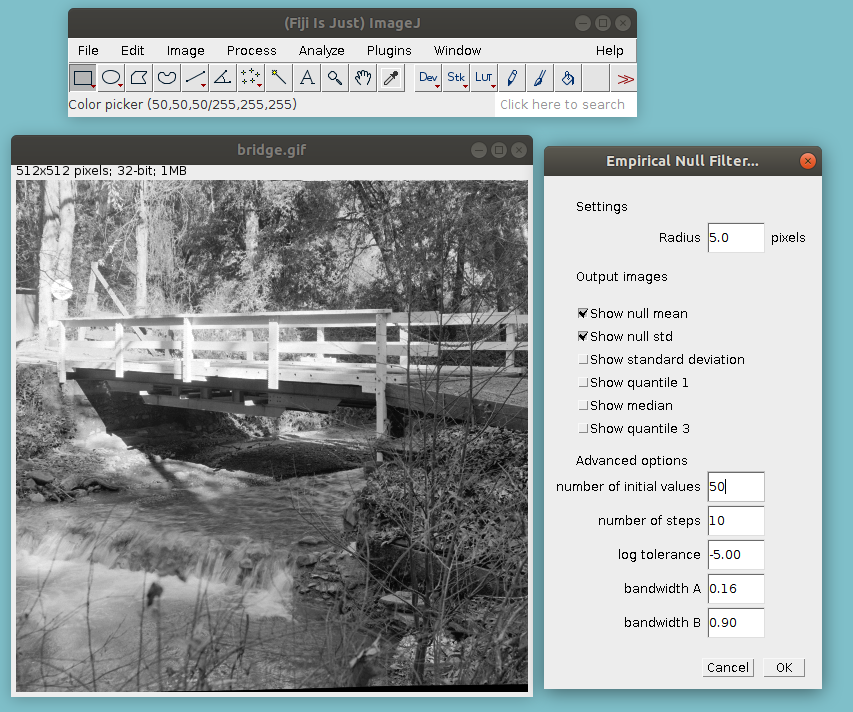
\includegraphics[width=\textwidth]{../figures/inference/fiji/gui.png}
    \caption{The graphical user interface of the empirical null filter in \emph{Fiji}. The user can adjust the kernel radius as well as other advanced options relating to the Newton-Raphson method and the kernel density estimate. By-products such as the empirical null parameters can be shown after the filtering as well.}
    \label{fig:inference_fijiGui}
\end{figure}

As a test, the empirical null filter with $r=\SI{5}{\pixel}$ was used on a \emph{ImageJ} sample image \texttt{bridge.gif}, as shown in Figure \ref{fig:inference_fijiBridgeFilter}. It is meaningless to use the empirical null filter on an arbitrary image, however, it did verify that the filter coped with it with some computational considerations. The empirical null images $\widehat{\mu}_{0,x,y}$ and $\widehat{\sigma}_{0,x,y}$ could be of interest, in particular, the empirical null mean image could be interpreted as the result of a mode filter \citep{griffin2000mean}. Figure \ref{fig:inference_fijiMean} compares the empirical null mean with other averaging filters. The empirical null mean has an impasto effect and preserved edges which are similar to the result in \cite{griffin2000mean}. Dispersion filters such as the standard deviation filter can be used to detect edges. Figure \ref{fig:inference_fijiStd} compares the standard deviation filter with the empirical null standard deviation. The resulting images were similar but it was notable that the edges in the empirical null standard deviation were sharper, suggesting that the empirical null standard deviation is a more robust measure of dispersion compared to the standard deviation.

\begin{figure}
  \centering
    \centerline{
    \begin{subfigure}[b]{\subSize}
        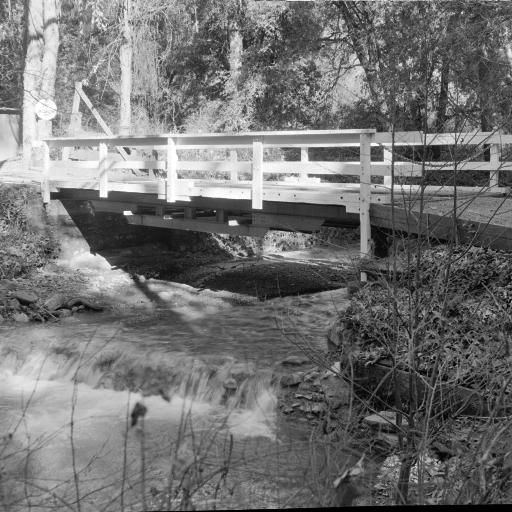
\includegraphics[width=\textwidth]{../figures/inference/fiji/bridge.png}
        \caption{Before filtering}
    \end{subfigure}
    \begin{subfigure}[b]{\subSize}
        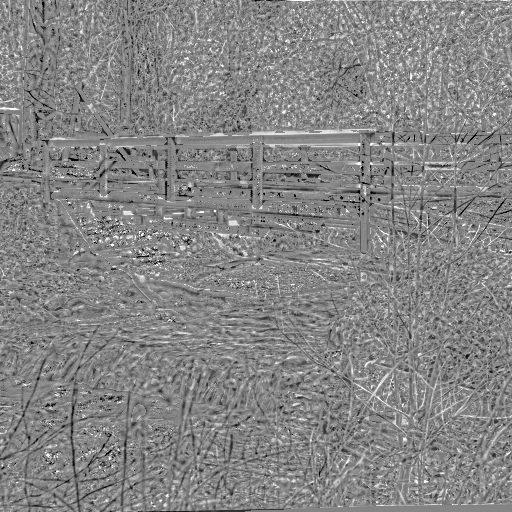
\includegraphics[width=\textwidth]{../figures/inference/fiji/bridgeFilter.png}
        \caption{After filtering}
    \end{subfigure}
    }
    \caption{The empirical null filter, with kernel radius $r=\SI{5}{\pixel}$, was used on the sample image \texttt{bridge.gif}.}
    \label{fig:inference_fijiBridgeFilter}
\end{figure}

\begin{figure}
  \centering
    \centerline{
    \begin{subfigure}[b]{\subSize}
        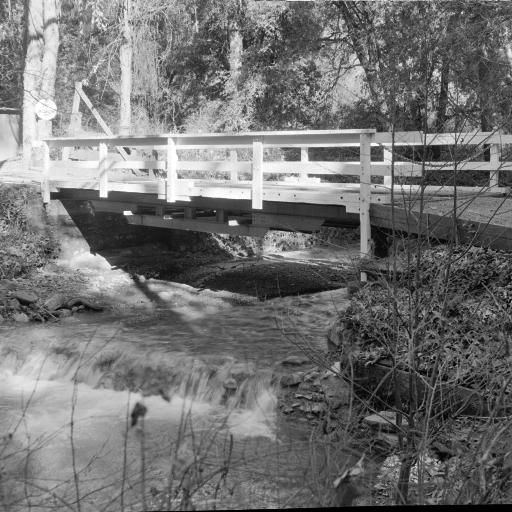
\includegraphics[width=\textwidth]{../figures/inference/fiji/bridge.png}
        \caption{No filter}
    \end{subfigure}
    \begin{subfigure}[b]{\subSize}
        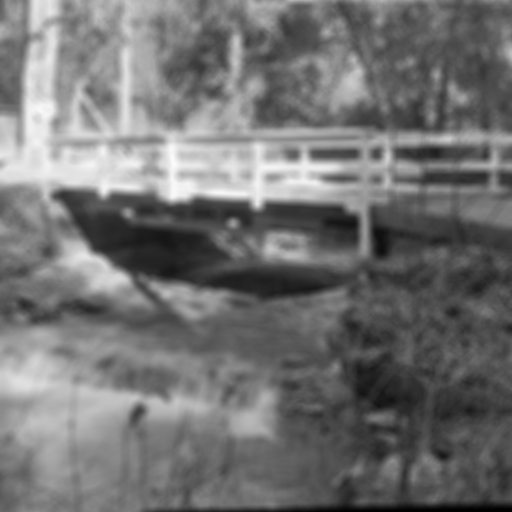
\includegraphics[width=\textwidth]{../figures/inference/fiji/mean.png}
        \caption{Mean filter}
    \end{subfigure}
    }
    \centerline{
    \begin{subfigure}[b]{\subSize}
        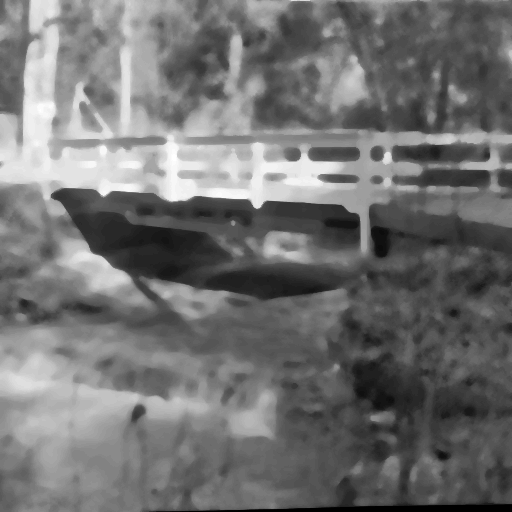
\includegraphics[width=\textwidth]{../figures/inference/fiji/median.png}
        \caption{Median filter}
    \end{subfigure}
    \begin{subfigure}[b]{\subSize}
        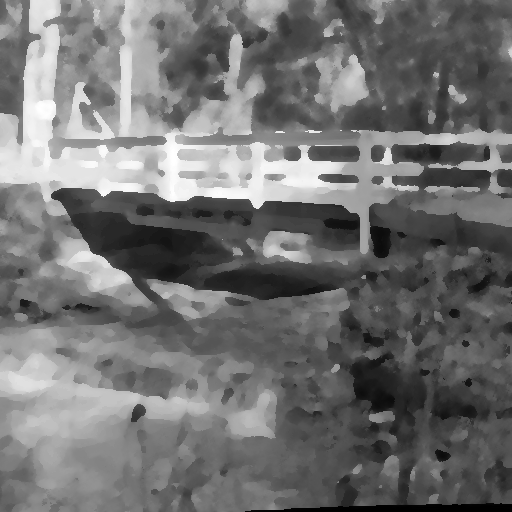
\includegraphics[width=\textwidth]{../figures/inference/fiji/nullMean.png}
        \caption{Empirical null mean}
    \end{subfigure}
    }
    \caption{Various averaging filters, with kernel radius $r=\SI{5}{\pixel}$, were used on the sample image \texttt{bridge.gif}.}
    \label{fig:inference_fijiMean}
\end{figure}

\begin{figure}
  \centering
    \centerline{
    \begin{subfigure}[b]{\subSize}
        \includegraphics[width=\textwidth]{../figures/inference/fiji/std.png}
        \caption{Standard deviation filter}
    \end{subfigure}
    \begin{subfigure}[b]{\subSize}
        \includegraphics[width=\textwidth]{../figures/inference/fiji/nullStd.png}
        \caption{Empirical null standard deviation}
    \end{subfigure}
    }
    \caption{Various dispersion filters, with kernel radius $r=\SI{5}{\pixel}$, were used on the sample image \texttt{bridge.gif}.}
    \label{fig:inference_fijiStd}
\end{figure}

When using the empirical null filter in \emph{ImageJ} or \emph{Fiji}, the user is presented with a menu, as shown in Figure \ref{fig:inference_fijiGui}. The user can input the kernel radius, the filter then modifies the currently selected image $z_{x,y}$ to $t_{x,y}$ for all $x$ and $y$ using a circular kernel with the specified radius. The menu also has options for by-product images to be shown: the empirical null mean $\widehat{\mu}_{0,x,y}$, the empirical null standard deviation $\widehat{\sigma}_{0,x,y}$, the standard deviation filter, quartile filters. Advanced options are available to the user, for example, the number of initial values set the number of valid solutions to be found when using the Newton-Raphson method to find the mode of the density estimate. The user can also set the maximum number of steps and tolerance for the Newton-Raphson method. The bandwidth parameters for the kernel density estimate can also be adjusted here.

Line filtering was done from left to right. At the start on the far left, an initial value of the median over the pixels in the kernel was used. Also, various initial values were randomly tried out until a requested number of valid solutions were found. For the following pixel to the right, the empirical null mean of the neighbouring left pixel was used as the initial value. This was chosen as it was assumed the empirical null mean would vary slowly and smoothly spatially. The implementation uses multiple threads, each thread filters a row in parallel.

When the kernel captures pixels outside the boundary of the image or ROI, \texttt{RankFilters} uses nearest pixel padding which fills in pixels outside the ROI with values to the nearest pixels. Figure \ref{fig:inference_padding_nearest} shows an example of nearest pixel padding on the top left corner of a rectangle ROI. This is not suitable for the empirical null filter as this will cause bias in the density estimation. The empirical null filter uses \texttt{NaN} padding which fills pixels outside the ROI with \texttt{NaN}. This indicates that these pixels are outside the ROI and are ignored. The number of non-\texttt{NaN} captured by the kernel was kept track for calculations such as the bandwidth.

\begin{figure}
  \centering
  \begin{subfigure}[b]{\subSize}
      \begin{tabular}{lllllll}
         $\ddots$ & $\vdots$ & $\vdots$ & $\vdots$ & $\vdots$ & $\udots$ \\
         $\dotsc$ & $z_{1,1}$ & $z_{1,1}$ & $z_{1,1}$ & $z_{1,2}$ & $\dotsc$ \\
         $\dotsc$ & $z_{1,1}$ & $z_{1,1}$ & $z_{1,1}$ & $z_{1,2}$ & $\dotsc$ \\ \cline{4-6}
         $\dotsc$ & $z_{1,1}$ & \multicolumn{1}{l|}{$z_{1,1}$} & $z_{1,1}$ & $z_{1,2}$ & $\dotsc$ \\
         $\dotsc$ & $z_{2,1}$ & \multicolumn{1}{l|}{$z_{2,1}$}  & $z_{2,1}$ & $z_{2,2}$ & $\dotsc$ \\
         $\udots$ & $\vdots$ & \multicolumn{1}{l|}{$\vdots$}  & $\vdots$ & $\vdots$ & $\ddots$
    \end{tabular}
    \caption{Nearest pixel padding}
    \label{fig:inference_padding_nearest}
  \end{subfigure}
  \begin{subfigure}[b]{\subSize}
      \begin{tabular}{lllllll}
         $\ddots$ & $\vdots$ & $\vdots$ & $\vdots$ & $\vdots$ & $\udots$ \\
         $\dotsc$ & \texttt{NaN} & \texttt{NaN} & \texttt{NaN} & \texttt{NaN} & $\dotsc$ \\
         $\dotsc$ & \texttt{NaN} & \texttt{NaN} & \texttt{NaN} & \texttt{NaN} & $\dotsc$ \\ \cline{4-6}
         $\dotsc$ & \texttt{NaN} & \multicolumn{1}{l|}{\texttt{NaN}} & $z_{1,1}$ & $z_{1,2}$ & $\dotsc$ \\
         $\dotsc$ & \texttt{NaN} & \multicolumn{1}{l|}{\texttt{NaN}}  & $z_{2,1}$ & $z_{2,2}$ & $\dotsc$ \\
         $\udots$ & $\vdots$ & \multicolumn{1}{l|}{$\vdots$}  & $\vdots$ & $\vdots$ & $\ddots$
    \end{tabular}
    \caption{\texttt{NaN} padding}
    \label{fig:inference_padding_nan}
  \end{subfigure}
  \caption{When a kernel contains pixels outside the ROI, as shown by the solid line, the pixels can either be extrapolated using the nearest pixel or completely ignored by filling in the missing pixels with \texttt{NaN}.}
  \label{fig:inference_padding}
\end{figure}

When filtering arbitrary images such as \texttt{bridge.gif}, a few computational considerations were needed. \texttt{bridge.gif} is an 8-bit image so values were represented as integers. This opened up opportunities for the interquartile range and the standard deviation to be zero. This caused problems as this would set the bandwidth to zero. When the standard deviation is zero, it was set to $0.289$ which corresponds to the standard deviation of a uniform random variable. When the inter-quartile range is zero, the inter-quartile range was set to the standard deviation $\times 1.34$.

When the number of initial values is too few, poor solutions to $\widehat{\mu}_0$ are possible which then can propagate to the pixel to the right and used as its initial value. Poor initial values could cause the Newton-Raphson method to never converge. If the Newton-Raphson method failed to converge too many times, the median, over pixels in the kernel, is used as the new initial value. Should it fail too, the program gives up and puts a $\texttt{NaN}$ in that pixel.

\subsection{Filtering an Image with No Defects}

An experiment was conducted to demonstrate the effects of the empirical null filter on a simulated $\SI{256}{\pixel}\times\SI{256}{\pixel}$ Gaussian image, where all the pixels have value distributed as standard Normal. The purpose is to simulate test statistics which are null and few positive results, subject to the FDR, should be detected. The test statistics after filtering should preserve its original distribution, or at least close to it. The statistical moments before and after filtering should be the same and were investigated. Because the empirical null mean and empirical null standard deviation are random variables, the filtered pixels will never be Normal and any normality tests would be too strict for this experiment.

Contamination is defined as some smooth and slowly varying function added and/or multiplied to an image. Conducting hypotheses testing on a contaminated Gaussian image may cause errors if the null distributions were incorrectly specified as standard Normal. In this experiment, the contamination was a gradient such that the pixel at position $(x,y)$ has a value distributed as $Z_{x,y}\sim\normal(\mu_{0,x,y},\sigma_{0,x,y}^2)$ where
\begin{equation}
  \mu_{0,x,y} = 0.01 (x-x_0) + 0.01 (y-y_0) \ ,
\end{equation}
$(x_0,y_0)$ is the centre of the image and $\sigma_{0,x,y}=2$ for all $(x,y)$.

A caveat is that some bias to the null standard deviation estimation would be introduced because of the contamination. This is because sources of variance captured by the kernel are from $\sigma_{0,x,y}$ and also from the variability of $\mu_{0,x,y}$. This can be shown with an example. Let $Z_{x,y}$ be the value of the pixels captured by the circular kernel, centred at the origin, for integer values of $(x,y)$ such that $x^2+y^2\leqslant r^2$. Suppose that $Z_{x,y}\sim\normal(ax+by,\sigma^2)$. The quantities of interest are the expectation and variance of all the values contained in the kernel because this is the quantity the estimators are estimating.

The calculations of the expectation and variance of $Z_{x,y}$ can be approximated by treating $x$ and $y$ as uniformly distributed within a circle centred at the origin with radius $r$. The expectation is
\begin{equation}
\expectation[Z_{X,Y}] = \expectation\expectation[Z_{X,Y}|X,Y]=0 \ .
\end{equation}

The variance is given as $\variance[Z_{X,Y}] = \expectation\variance[Z_{X,Y}|X,Y] + \variance\expectation[Z_{X,Y}|X,Y]$. From the distribution of $Z_{X,Y}$, $\expectation\variance[Z_{X,Y}|X,Y] = \sigma^2$ and $\variance\expectation[Z_{X,Y}|X,Y]=\variance[aX+bY]$. This is worked out to be
\begin{align}
\variance[aX+bY] &= \dfrac{1}{\pi r^2}\int_{\rho=0}^{\rho=r}\int_{\theta=0}^{\theta=2\pi}
\rho^3(a\cos\theta + b\sin\theta)^2 \diff \theta \diff \rho
\nonumber\\
& = \dfrac{1}{4}(a^2+b^2)r^2
\end{align}
thus
\begin{equation}
\variance[Z_{X,Y}] = \dfrac{1}{4}(a^2+b^2)r^2 + \sigma^2 \ .
\end{equation}
This shows that when estimating the null variance on a contaminated Gaussian image, there may be a $(a^2+b^2)r^2/4$ bias. If the contamination is slowly varying, that is $a$ and $b$ are small, then the bias should be small.

\begin{figure}[p]
  \centering
  \centerline{
  \begin{subfigure}[b]{\subSize}
    \includegraphics[width=\textwidth]{../figures/inference/allNullGaussianScript_beforeFilter.eps}
    \caption{Unfiltered}
  \end{subfigure}
  \begin{subfigure}[b]{\subSize}
    \includegraphics[width=\textwidth]{../figures/inference/allNullGaussianScript_afterFilter.eps}
    \caption{Filtered}
    \label{fig:inference_allNullGaussianScript_afterFilter}
  \end{subfigure}
  }
  \centerline{
  \begin{subfigure}[b]{\subSize}
    \includegraphics[width=\textwidth]{../figures/inference/allNullGaussianScript_nullMean.eps}
    \caption{Empirical null mean}
  \end{subfigure}
  \begin{subfigure}[b]{\subSize}
    \includegraphics[width=\textwidth]{../figures/inference/allNullGaussianScript_nullStd.eps}
    \caption{Empirical null std}
  \end{subfigure}
  }
  \caption{A $\SI{256}{\pixel}\times \SI{256}{\pixel}$ Gaussian image before and after filtering with kernel radius \SI{20}{\pixel}. Also shown are the empirical null mean and empirical null standard deviation.}
  \label{fig:inference_allNullGaussianScript}
\end{figure}

\begin{figure}[p]
  \centering
  \centerline{
  \begin{subfigure}[b]{\subSize}
    \includegraphics[width=\textwidth]{../figures/inference/allNullPlaneScript_beforeFilter.eps}
    \caption{Unfiltered}
  \end{subfigure}
  \begin{subfigure}[b]{\subSize}
    \includegraphics[width=\textwidth]{../figures/inference/allNullPlaneScript_afterFilter.eps}
    \caption{Filtered}
    \label{fig:inference_allNullPlaneScript_afterFilter}
  \end{subfigure}
  }
  \centerline{
  \begin{subfigure}[b]{\subSize}
    \includegraphics[width=\textwidth]{../figures/inference/allNullPlaneScript_nullMean.eps}
    \caption{Empirical null mean}
  \end{subfigure}
  \begin{subfigure}[b]{\subSize}
    \includegraphics[width=\textwidth]{../figures/inference/allNullPlaneScript_nullStd.eps}
    \caption{Empirical null std}
  \end{subfigure}
  }
  \caption{A $\SI{256}{\pixel}\times \SI{256}{\pixel}$ contaminated Gaussian image before and after filtering with kernel radius \SI{20}{\pixel}. The contamination was such that the null distribution is $Z_{x,y}|H_{0,x,y}\sim\normal(\mu_{0,x,y},\sigma_0^2)$ where $\mu_{0,x,y} = 0.01 (x-x_0) + 0.01 (y-y_0)$ and $\sigma_0=2$. Also shown are the empirical null mean and empirical null standard deviation.}
  \label{fig:inference_allNullPlaneScript}
\end{figure}

\begin{figure}
  \centering
  \begin{subfigure}[b]{\subSize}
    \includegraphics[width=\textwidth]{../figures/inference/allNullGaussianScript_pValue.eps}
    \caption{No contamination}
  \end{subfigure}
  \begin{subfigure}[b]{\subSize}
    \includegraphics[width=\textwidth]{../figures/inference/allNullPlaneScript_pValue.eps}
    \caption{With contamination}
  \end{subfigure}
  \caption{$p$-values from a filtered $\SI{256}{\pixel}\times \SI{256}{\pixel}$ Gaussian image with kernel radius \SI{20}{\pixel}. In b), the Gaussian image was contaminated before filtering. The contamination was such that the null distribution is $Z_{x,y}|H_{0,x,y}\sim\normal(\mu_{0,x,y},\sigma_0^2)$ where $\mu_{0,x,y} = 0.01 (x-x_0) + 0.01 (y-y_0)$ and $\sigma_0=2$. The $p$-values were obtained from the images in Figures \ref{fig:inference_allNullGaussianScript_afterFilter} and \ref{fig:inference_allNullPlaneScript_afterFilter}. The critical region corresponds to the 5\% FDR level. The dotted lines shows the $p$-values if they were uniformly distributed.}
  \label{fig:inference_allNull_pValues}
\end{figure}

An example of a Gaussian image with/without contamination before/after filtering are shown in Figures \ref{fig:inference_allNullGaussianScript} and \ref{fig:inference_allNullPlaneScript}. In the contaminated example, the filter managed to estimate the null mean, picking up the gradient. This enabled the filtered image to look flat and removed the contamination. The $p$-values after filtering are shown in Figure \ref{fig:inference_allNull_pValues}. A quick inspection suggests that the filtered pixels appeared reasonably Normal for this particular example.

For a given kernel radius $r$, 100 different Gaussian images were filtered to investigate the within image mean, standard deviation and kurtosis of the filtered statistics. Various other filters for normalisation were used as well such as the MADA-mode null filter, median IQR null filter and the mean variance null filter. They use different estimators to estimate the null parameters as their name suggests, Table \ref{table:inference_nullFilters} clarifies them.

\begin{table}
  \centering
  \begin{tabular}{l|l|l}
    Filters&Null mean&Null standard deviation\\\hline
    MADA-mode null&Mode&MADA-mode $\times1.483$\\
    Median IQR null&Median&IQR $\div1.349$\\
    Mean variance null&Mean&Standard deviation
  \end{tabular}
  \caption{Various filters using different estimators to estimate the null parameters are described here.}
  \label{table:inference_nullFilters}
\end{table}

\begin{figure}
  \centering
  \centerline{
  \begin{subfigure}[b]{\subSize}
    \includegraphics[width=\textwidth]{../figures/inference/AllNullGaussianEmpirical_mean.eps}
    \caption{Empirical null filter}
  \end{subfigure}
  \begin{subfigure}[b]{\subSize}
    \includegraphics[width=\textwidth]{../figures/inference/AllNullGaussianMadMode_mean.eps}
    \caption{MADA-mode null filter}
  \end{subfigure}
  }
  \centerline{
    \begin{subfigure}[b]{\subSize}
    \includegraphics[width=\textwidth]{../figures/inference/AllNullGaussianMedianIqr_mean.eps}
    \caption{Median IQR null filter}
  \end{subfigure}
  \begin{subfigure}[b]{\subSize}
    \includegraphics[width=\textwidth]{../figures/inference/AllNullGaussianMeanVar_mean.eps}
    \caption{Mean var null filter}
  \end{subfigure}
  }
  \caption{The within image sample mean of a filtered Gaussian image of size $\SI{256}{\pixel}\times\SI{256}{\pixel}$.  The boxplots summarise the 100 repeated simulations of the image. The dashed lines show the 95\% confidence interval using standard tests and assuming independence.}
  \label{fig:inference_AllNullGaussian_mean}
\end{figure}

\begin{figure}
  \centering
  \centerline{
  \begin{subfigure}[b]{\subSize}
    \includegraphics[width=\textwidth]{../figures/inference/AllNullGaussianEmpirical_variance.eps}
    \caption{Empirical null filter}
  \end{subfigure}
  \begin{subfigure}[b]{\subSize}
    \includegraphics[width=\textwidth]{../figures/inference/AllNullGaussianMadMode_variance.eps}
    \caption{MADA-mode null filter}
  \end{subfigure}
  }
  \centerline{
    \begin{subfigure}[b]{\subSize}
    \includegraphics[width=\textwidth]{../figures/inference/AllNullGaussianMedianIqr_variance.eps}
    \caption{Median IQR null filter}
  \end{subfigure}
  \begin{subfigure}[b]{\subSize}
    \includegraphics[width=\textwidth]{../figures/inference/AllNullGaussianMeanVar_variance.eps}
    \caption{Mean var null filter}
  \end{subfigure}
  }
  \caption{The within image sample standard deviation of a filtered Gaussian image of size $\SI{256}{\pixel}\times\SI{256}{\pixel}$. The boxplots summarise the 100 repeated simulations of the image. The dashed lines show the 95\% confidence interval using standard tests and assuming independence.}
  \label{fig:inference_AllNullGaussian_var}
\end{figure}

\begin{figure}
  \centering
  \centerline{
  \begin{subfigure}[b]{\subSize}
    \includegraphics[width=\textwidth]{../figures/inference/AllNullGaussianEmpirical_kurtosis.eps}
    \caption{Empirical null filter}
  \end{subfigure}
  \begin{subfigure}[b]{\subSize}
    \includegraphics[width=\textwidth]{../figures/inference/AllNullGaussianMadMode_kurtosis.eps}
    \caption{MADA-mode null filter}
  \end{subfigure}
  }
  \centerline{
    \begin{subfigure}[b]{\subSize}
    \includegraphics[width=\textwidth]{../figures/inference/AllNullGaussianMedianIqr_kurtosis.eps}
    \caption{Median IQR null filter}
  \end{subfigure}
  \begin{subfigure}[b]{\subSize}
    \includegraphics[width=\textwidth]{../figures/inference/AllNullGaussianMeanVar_kurtosis.eps}
    \caption{Mean var null filter}
  \end{subfigure}
  }
  \caption{The within image sample kurtosis of a filtered Gaussian image of size $\SI{256}{\pixel}\times\SI{256}{\pixel}$. The boxplots summarise the 100 repeated simulations of the image. The dashed lines show the 95\% confidence interval using standard tests and assuming independence.}
  \label{fig:inference_AllNullGaussian_kurtosis}
\end{figure}

\begin{figure}
  \centering
  \centerline{
  \begin{subfigure}[b]{\subSize}
    \includegraphics[width=\textwidth]{../figures/inference/AllNullPlaneEmpirical_mean.eps}
    \caption{Empirical null filter}
  \end{subfigure}
  \begin{subfigure}[b]{\subSize}
    \includegraphics[width=\textwidth]{../figures/inference/AllNullPlaneMadMode_mean.eps}
    \caption{MADA-mode null filter}
  \end{subfigure}
  }
  \centerline{
    \begin{subfigure}[b]{\subSize}
    \includegraphics[width=\textwidth]{../figures/inference/AllNullPlaneMedianIqr_mean.eps}
    \caption{Median IQR null filter}
  \end{subfigure}
  \begin{subfigure}[b]{\subSize}
    \includegraphics[width=\textwidth]{../figures/inference/AllNullPlaneMeanVar_mean.eps}
    \caption{Mean var null filter}
  \end{subfigure}
  }
  \caption{The within image sample mean of a filtered contaminated Gaussian image of size $\SI{256}{\pixel}\times\SI{256}{\pixel}$. The contamination was such that the null distribution is $Z_{x,y}|H_{0,x,y}\sim\normal(\mu_{0,x,y},\sigma_0^2)$ where $\mu_{0,x,y} = 0.01 (x-x_0) + 0.01 (y-y_0)$ and $\sigma_0=2$. The boxplots summarise the 100 repeated simulations of the image. The dashed lines show the 95\% confidence interval using standard tests and assuming independence.}
  \label{fig:inference_AllNullPlane_mean}
\end{figure}

\begin{figure}
  \centering
  \centerline{
  \begin{subfigure}[b]{\subSize}
    \includegraphics[width=\textwidth]{../figures/inference/AllNullPlaneEmpirical_variance.eps}
    \caption{Empirical null filter}
  \end{subfigure}
  \begin{subfigure}[b]{\subSize}
    \includegraphics[width=\textwidth]{../figures/inference/AllNullPlaneMadMode_variance.eps}
    \caption{MADA-mode null filter}
  \end{subfigure}
  }
  \centerline{
    \begin{subfigure}[b]{\subSize}
    \includegraphics[width=\textwidth]{../figures/inference/AllNullPlaneMedianIqr_variance.eps}
    \caption{Median IQR null filter}
  \end{subfigure}
  \begin{subfigure}[b]{\subSize}
    \includegraphics[width=\textwidth]{../figures/inference/AllNullPlaneMeanVar_variance.eps}
    \caption{Mean var null filter}
  \end{subfigure}
  }
  \caption{The within image sample standard deviation of a filtered contaminated Gaussian image of size $\SI{256}{\pixel}\times\SI{256}{\pixel}$. The contamination was such that the null distribution is $Z_{x,y}|H_{0,x,y}\sim\normal(\mu_{0,x,y},\sigma_0^2)$ where $\mu_{0,x,y} = 0.01 (x-x_0) + 0.01 (y-y_0)$ and $\sigma_0=2$. The boxplots summarise the 100 repeated simulations of the image. The dashed lines show the 95\% confidence interval using standard tests and assuming independence.}
  \label{fig:inference_AllNullPlane_var}
\end{figure}

\begin{figure}
  \centering
  \centerline{
  \begin{subfigure}[b]{\subSize}
    \includegraphics[width=\textwidth]{../figures/inference/AllNullPlaneEmpirical_kurtosis.eps}
    \caption{Empirical null filter}
  \end{subfigure}
  \begin{subfigure}[b]{\subSize}
    \includegraphics[width=\textwidth]{../figures/inference/AllNullPlaneMadMode_kurtosis.eps}
    \caption{MADA-mode null filter}
  \end{subfigure}
  }
  \centerline{
    \begin{subfigure}[b]{\subSize}
    \includegraphics[width=\textwidth]{../figures/inference/AllNullPlaneMedianIqr_kurtosis.eps}
    \caption{Median IQR null filter}
  \end{subfigure}
  \begin{subfigure}[b]{\subSize}
    \includegraphics[width=\textwidth]{../figures/inference/AllNullPlaneMeanVar_kurtosis.eps}
    \caption{Mean var null filter}
  \end{subfigure}
  }
  \caption{The within image sample kurtosis of a filtered contaminated Gaussian image of size $\SI{256}{\pixel}\times\SI{256}{\pixel}$. The contamination was such that the null distribution is $Z_{x,y}|H_{0,x,y}\sim\normal(\mu_{0,x,y},\sigma_0^2)$ where $\mu_{0,x,y} = 0.01 (x-x_0) + 0.01 (y-y_0)$ and $\sigma_0=2$. The boxplots summarise the 100 repeated simulations of the image. The dashed lines show the 95\% confidence interval using standard tests and assuming independence.}
  \label{fig:inference_AllNullPlane_kurtosis}
\end{figure}

The results for the filtered images are shown in Figures \ref{fig:inference_AllNullGaussian_mean}, \ref{fig:inference_AllNullGaussian_var} and \ref{fig:inference_AllNullGaussian_kurtosis}. For the filtered contaminated images, they are in Figures \ref{fig:inference_AllNullPlane_mean}, \ref{fig:inference_AllNullPlane_var} and \ref{fig:inference_AllNullPlane_kurtosis}. The filtered test statistic means did agree with zero as expected, showing that the filters centred the statistics when normalising. When using the empirical null filter, there was some negative bias with the standard deviation of the filtered test statistics. The negative bias comes from a positive bias when estimating the null standard deviation.

When filtering the contaminated image, all estimators suffered from negative bias in the standard deviation of the filtered statistics, in particular when the kernel radius increased. This is shown in Figure \ref{fig:inference_AllNullPlane_var}. As discussed before, the kernel captured the variation due to the contamination and this added bias to the estimation of the null standard deviation.

The kurtosis in Figures \ref{fig:inference_AllNullGaussian_kurtosis} and \ref{fig:inference_AllNullPlane_kurtosis} showed that the empirical null filter caused the filtered statistics to have heavy tails, in particular, for small kernel radiuses. This could cause problems in hypotheses testing because heavy tails could be misinterpreted as a contribution from non-null statistics. The source of the kurtosis inflation is from the estimation of the null standard deviation. This can be seen by comparing the empirical null filter with the MADA-mode null filter because the only difference between the two filters is in the estimation of the null standard deviation.

\afterpage{\clearpage}
\subsection{Detection of Simulated Defects}

The empirical null filter was tested to see if it can assist in detecting simulated defects from an image with/without contamination. A defect assigns pixels to have a value not distributed under the null distribution, but instead, under an alternative, or non-null, distribution. For example, suppose $Z_{x,y}|H_{0,x,y}\sim\normal(0,1)$, then a defect assign certain pixels to have a value distributed as $Z_{x,y}|H_{1,x,y}\sim\normal(\mu_{1},1)$ where $\mu_1\neq0$.

To recap, contamination is the result of a linear transform of the test statistics $Z_{x,y}$. For example, in this experiment, the image was multiplied by 2 and a gradient was added to it. The resulting null and alternative distributions are
\begin{align}
  Z_{x,y}|H_{0,x,y}&\sim\normal(\mu_{0,x,y},2^2)
  \\
  Z_{x,y}|H_{1,x,y}&\sim\normal(2\mu_1+\mu_{0,x,y},2^2)
\end{align}
respectively where $\mu_{0,x,y}=0.01(x-x_0)+0.01(y-y_0)$ and $(x_0,y_0)$ is the centre of the image. This was used in this experiment to simulate a contaminated image with defects.

The empirical null filter aims to estimate the null distribution parameters from $Z_{x,y}$ to normalise it to form $T_{x,y}$. By normalising it, $T_{x,y}|H_{0,x,y}$ should be approximately standard Normal and hypotheses testing can be used to detect defects.

Various defects were investigated. Speckle defect with density $\pi_1$ assign all test statistics to be non-null with probability $\pi_1$ and are null otherwise. This was chosen because the proportion of null statistics captured by the kernel should be the same for all kernel radiuses. A line defect assigns columns of pixels to be non-null, a kernel would only capture a section of the defect. A square defect was also investigated and a kernel can capture the entire defect only if its radius is large enough.

\begin{figure}[p]
  \centering
    \centerline{
      \begin{subfigure}{\subSize}
        \includegraphics[width=\textwidth]{../figures/inference/DefectExampleDust_imageClean.eps}
        \caption{Uncontaminated}
      \end{subfigure}
      \begin{subfigure}{\subSize}
        \includegraphics[width=\textwidth]{../figures/inference/DefectExampleDust_imageContaminated.eps}
        \caption{Contaminated}
      \end{subfigure}
    }
    \centerline{
      \begin{subfigure}{\subSize}
        \includegraphics[width=\textwidth]{../figures/inference/DefectExampleDust_EmpiricalNullFilterimageFiltered.eps}
        \caption{Filtered}
      \end{subfigure}
      \begin{subfigure}{\subSize}
        \includegraphics[width=\textwidth]{../figures/inference/DefectExampleDust_EmpiricalNullFilternullStd.eps}
        \caption{Empirical null std}
      \end{subfigure}
    }
  \caption{A $\SI{256}{\pixel} \times \SI{256}{\pixel}$ Gaussian image with speckle defect is shown in a). The image was contaminated in b) and then filtered with kernel radius \SI{20}{\pixel} in c). Non-null pixels have the distribution $\normal(3,1)$. The speckle defect has density $\pi_1 = 0.1$. The contamination was such that the null distribution is $Z_{x,y}|H_{0,x,y}\sim\normal(\mu_{0,x,y},\sigma_0^2)$ where $\mu_{0,x,y} = 0.01 (x-x_0) + 0.01 (y-y_0)$ and $\sigma_0=2$. In a), c) and d), highlighted in red are pixels tested as positive at the 5\% FDR level.}
  \label{fig:inference_defectDustExample}
\end{figure}

\begin{figure}[p]
  \centering
    \centerline{
      \begin{subfigure}{\subSize}
        \includegraphics[width=\textwidth]{../figures/inference/DefectExampleLine_imageClean.eps}
        \caption{Uncontaminated}
      \end{subfigure}
      \begin{subfigure}{\subSize}
        \includegraphics[width=\textwidth]{../figures/inference/DefectExampleLine_imageContaminated.eps}
        \caption{Contaminated}
      \end{subfigure}
    }
    \centerline{
      \begin{subfigure}{\subSize}
        \includegraphics[width=\textwidth]{../figures/inference/DefectExampleLine_EmpiricalNullFilterimageFiltered.eps}
        \caption{Filtered}
      \end{subfigure}
      \begin{subfigure}{\subSize}
        \includegraphics[width=\textwidth]{../figures/inference/DefectExampleLine_EmpiricalNullFilternullStd.eps}
        \caption{Empirical null std}
      \end{subfigure}
    }
  \caption{A $\SI{256}{\pixel} \times \SI{256}{\pixel}$ Gaussian image with a line defect is shown in a). The image was contaminated in b) and then filtered with kernel radius \SI{20}{\pixel} in c). Non-null pixels have the distribution $\normal(3,1)$. The line defect is \SI{5}{\pixel} thick. The contamination was such that the null distribution is $Z_{x,y}|H_{0,x,y}\sim\normal(\mu_{0,x,y},\sigma_0^2)$ where $\mu_{0,x,y} = 0.01 (x-x_0) + 0.01 (y-y_0)$ and $\sigma_0=2$. In a), c) and d), highlighted in red are pixels tested as positive at the 5\% FDR level.}
  \label{fig:inference_defectLineExample}
\end{figure}

\begin{figure}[p]
  \centering
    \centerline{
      \begin{subfigure}{\subSize}
        \includegraphics[width=\textwidth]{../figures/inference/DefectExampleSquare20_imageClean.eps}
        \caption{Uncontaminated}
      \end{subfigure}
      \begin{subfigure}{\subSize}
        \includegraphics[width=\textwidth]{../figures/inference/DefectExampleSquare20_imageContaminated.eps}
        \caption{Contaminated}
      \end{subfigure}
    }
    \centerline{
      \begin{subfigure}{\subSize}
        \includegraphics[width=\textwidth]{../figures/inference/DefectExampleSquare20_EmpiricalNullFilterimageFiltered.eps}
        \caption{Filtered}
      \end{subfigure}
      \begin{subfigure}{\subSize}
        \includegraphics[width=\textwidth]{../figures/inference/DefectExampleSquare20_EmpiricalNullFilternullMean.eps}
        \caption{Empirical null mean}
      \end{subfigure}
    }
  \caption{A $\SI{256}{\pixel} \times \SI{256}{\pixel}$ Gaussian image with a square defect is shown in a). The image was contaminated in b) and then filtered with kernel radius \SI{20}{\pixel} in c). Non-null pixels have the distribution $\normal(3,1)$. The square defect is $\SI{30}{\pixel}\times \SI{30}{\pixel}$ in size. The contamination was such that the null distribution is $Z_{x,y}|H_{0,x,y}\sim\normal(\mu_{0,x,y},\sigma_0^2)$ where $\mu_{0,x,y} = 0.01 (x-x_0) + 0.01 (y-y_0)$ and $\sigma_0=2$. In a) and c), highlighted in red are pixels tested as positive at the 5\% FDR level.}
  \label{fig:inference_defectSquareExample}
\end{figure}

\begin{figure}[p]
  \centering
    \centerline{
      \begin{subfigure}{\subSize}
        \includegraphics[width=\textwidth]{../figures/inference/DefectExampleSquare40_imageClean.eps}
        \caption{Uncontaminated}
      \end{subfigure}
      \begin{subfigure}{\subSize}
        \includegraphics[width=\textwidth]{../figures/inference/DefectExampleSquare40_imageContaminated.eps}
        \caption{Contaminated}
      \end{subfigure}
    }
    \centerline{
      \begin{subfigure}{\subSize}
        \includegraphics[width=\textwidth]{../figures/inference/DefectExampleSquare40_EmpiricalNullFilterimageFiltered.eps}
        \caption{Filtered}
      \end{subfigure}
      \begin{subfigure}{\subSize}
        \includegraphics[width=\textwidth]{../figures/inference/DefectExampleSquare40_EmpiricalNullFilternullMean.eps}
        \caption{Empirical null mean}
      \end{subfigure}
    }
  \caption{A $\SI{256}{\pixel} \times \SI{256}{\pixel}$ Gaussian image with a square defect is shown in a). The image was contaminated in b) and then filtered with kernel radius \SI{40}{\pixel} in c). Non-null pixels have the distribution $\normal(3,1)$. The square defect is $\SI{30}{\pixel}\times \SI{30}{\pixel}$ in size. The contamination was such that the null distribution is $Z_{x,y}|H_{0,x,y}\sim\normal(\mu_{0,x,y},\sigma_0^2)$ where $\mu_{0,x,y} = 0.01 (x-x_0) + 0.01 (y-y_0)$ and $\sigma_0=2$. In a) and c), highlighted in red are pixels tested as positive at the 5\% FDR level.}
  \label{fig:inference_defectSquare2Example}
\end{figure}

\begin{figure}[p]
  \centering
    \centerline{
      \begin{subfigure}{\subSize}
        \includegraphics[width=\textwidth]{../figures/inference/DefectExampleDust_EmpiricalNullFilterpValueFiltered.eps}
        \caption{Speckle defect, $r=\SI{20}{\pixel}$}
      \end{subfigure}
      \begin{subfigure}{\subSize}
        \includegraphics[width=\textwidth]{../figures/inference/DefectExampleLine_EmpiricalNullFilterpValueFiltered.eps}
        \caption{Line defect, $r=\SI{20}{\pixel}$}
      \end{subfigure}
    }
    \centerline{
      \begin{subfigure}{\subSize}
        \includegraphics[width=\textwidth]{../figures/inference/DefectExampleSquare20_EmpiricalNullFilterpValueFiltered}
        \caption{Square defect, $r=\SI{20}{\pixel}$}
      \end{subfigure}
      \begin{subfigure}{\subSize}
        \includegraphics[width=\textwidth]{../figures/inference/DefectExampleSquare40_EmpiricalNullFilterpValueFiltered}
        \caption{Square defect, $r=\SI{40}{\pixel}$}
      \end{subfigure}
    }
  \caption{A $\SI{256}{\pixel} \times \SI{256}{\pixel}$ contamined defected Gaussian image was filtered using the empirical null filter with kernel radius $r$. Shown are the $p$-values converted from the filtered images. Non-null pixels have the distribution $\normal(3,1)$. The speckle defect has density $\pi_1=0.1$. The line defect is \SI{5}{\pixel} thick. The square defect is $\SI{30}{\pixel}\times \SI{30}{\pixel}$ in size. The contamination was such that the null distribution is $Z_{x,y}|H_{0,x,y}\sim\normal(\mu_{0,x,y},\sigma_0^2)$ where $\mu_{0,x,y} = 0.01 (x-x_0) + 0.01 (y-y_0)$ and $\sigma_0=2$. The critical region corresponds to the 5\% FDR level. The dotted lines shows the $p$-values if they were uniformly distributed.}
  \label{fig:inference_defectExamplePValue}
\end{figure}

An example of a speckle defected image is shown in Figure \ref{fig:inference_defectDustExample}, the figure also shows the image contaminated and then filtered. Without filtering, the top-left and bottom-right of the contaminated image have large, in magnitude, test statistics. In these areas, a lot of pixels would be tested as falsely positive. By using the empirical null filter, the resulting filtered image reassemble the uncontaminated image and appropriate inference can be done on the filtered image. However, some statistical power was lost when conducting hypotheses testing on the filtered image because, in areas of high empirical null standard deviation, the normalised statistics became too small which then decreased the detection power. This cannot be avoided as areas of high empirical null standard deviation was due to the randomness in sampling. Similar comments can be made for the line defect as shown in Figure \ref{fig:inference_defectLineExample}.

The square defected images, including the contaminated ones, are shown in Figures \ref{fig:inference_defectSquareExample} and \ref{fig:inference_defectSquare2Example}. Figure \ref{fig:inference_defectSquareExample} filtered the contaminated image using a kernel radius of $r=\SI{20}{\pixel}$, while Figure \ref{fig:inference_defectSquare2Example} used a kernel radius of $r=\SI{40}{\pixel}$. With $r=\SI{20}{\pixel}$, the kernel is smaller than the square defect, therefore, the defect was treated as the null. This is evident because the empirical null mean captured the defect. This resulted in difficulty detecting the defect. With $r=\SI{40}{\pixel}$, the kernel is bigger than the defect and treated the defect as non-null. In this scenario, the empirical null filter recovered the gradient in the empirical null which was then used for normalisation.

The empirical null mean in Figure \ref{fig:inference_defectSquareExample} demonstrated the multi-thread nature of the implementation of the empirical null filter. It can be seen that there were horizontal streaks where the defect is. This is the result of each thread filtering a row and jumping from one mode, the null, to the other, the non-null, at different times. The horizontal streaks can be removed by using more initial values so that the Newton-Raphson method can pinpoint which mode is greater. However, this would be at a computational cost.

Figure \ref{fig:inference_defectExamplePValue} shows the $p$-values after filtering a contaminated defected image. The FDR can be estimated in these figures by dividing the number of null statistics in the critical region by the number of statistics in the critical region. With a sensible kernel radius, some of the defects can be detected. False negatives are common but this is inevitable to control for the FDR. The figure shows that using a kernel radius of $r=\SI{20}{\pixel}$, for the square defect, failed to capture the defect. This, again, emphasise the importance of a good kernel radius.

The receiver operating characteristic (ROC) curves \citep{green1966signal, metz1978basic, hanley1982meaning, friedman2001elements, cook2007use} are shown in Figure \ref{fig:inference_defectSimulationRoc} for the various defects and filters. The ROC curve is a parametric plot, plotting the true positive rate (sensitivity) against the false positive rate ($1-\text{specificity}$) for varying thresholds. The area under the ROC curve (AUC) is a commonly used statistic to quantify the performance of the test \citep{friedman2001elements}. Interpretations of the area do exist \citep{metz1978basic,hanley1982meaning} and discussed thoroughly in \cite{cook2007use}.

\begin{figure}
  \centering
    \centerline{
      \begin{subfigure}{\subSize}
        \includegraphics[width=\textwidth]{../figures/inference/DefectExampleDust_roc.eps}
        \caption{Speckle defect, $r=\SI{20}{\pixel}$}
      \end{subfigure}
      \begin{subfigure}{\subSize}
        \includegraphics[width=\textwidth]{../figures/inference/DefectExampleLine_roc.eps}
        \caption{Line defect, $r=\SI{20}{\pixel}$}
      \end{subfigure}
    }
    \centerline{
      \begin{subfigure}{\subSize}
        \includegraphics[width=\textwidth]{../figures/inference/DefectExampleSquare20_roc.eps}
        \caption{Square defect, $r=\SI{20}{\pixel}$}
        \label{fig:inference_defectSimulationRoc_square20}
      \end{subfigure}
      \begin{subfigure}{\subSize}
        \includegraphics[width=\textwidth]{../figures/inference/DefectExampleSquare40_roc.eps}
        \caption{Square defect, $r=\SI{40}{\pixel}$}
      \end{subfigure}
    }
  \caption{ROC curves for various defected $\SI{256}{\pixel}\times \SI{256}{\pixel}$ Gaussian images. The upper/lower dot-dashed lines show the resulting ROC curve when testing on an image without/with contamination respectively. The different curves are the resulting ROC curves after filtering a contaminated image. The speckle defect has density $\pi_1=0.1$. The line defect is \SI{5}{\pixel} thick. The square defect is $\SI{30}{\pixel}\times \SI{30}{\pixel}$ in size. Defected pixels have the distribution $\normal(3,1)$. The contamination was such that the null distribution is $Z_{x,y}|H_{0,x,y}\sim\normal(\mu_{0,x,y},\sigma_0^2)$ where $\mu_{0,x,y} = 0.01 (x-x_0) + 0.01 (y-y_0)$ and $\sigma_0=2$.}
  \label{fig:inference_defectSimulationRoc}
\end{figure}

In terms of the AUC, the empirical null filter improved the performance of hypotheses testing compared with using the unfiltered contaminated image. The performance before contamination cannot be recovered but it was an improvement. For kernel radiuses too small, such as Figure \ref{fig:inference_defectSimulationRoc_square20}, the empirical null filter deteriorated the performance and it would be better off using the contaminated image.

\subsection{Speckle Defect Experiment}

The ROC curves consider all thresholds or specificities used in the hypotheses testing. In the previous experiment, it was found that the variance of the test statistics was different before and after filtering. As a result, for a given threshold, such as the 5\% FDR level, the specificity may change ever so slightly after filtering.

An experiment was conducted to investigate how filtering affects hypotheses testing. A $\SI{256}{\pixel}\times \SI{256}{\pixel}$ Gaussian image with speckle defect, with density $\pi_1=0.1$, and various values of $\mu_1$ were investigated. The AUC, type 1 error, type 2 error and FDR were measured when testing on an image with a defect before and after contamination and then after filtering with the contamination. The AUC was obtained by integrating the ROC curve. A kernel radius of $r=\SI{20}{\pixel}$ was used and was repeated 100 times by simulating another image.

\begin{figure}
  \centering
    \centerline{
      \begin{subfigure}{\subSize}
        \includegraphics[width=\textwidth]{../figures/inference/DefectAltDustEmpirical_roc.eps}
        \caption{AUC}
      \end{subfigure}
      \begin{subfigure}{\subSize}
        \includegraphics[width=\textwidth]{../figures/inference/DefectAltDustEmpirical_type1.eps}
        \caption{Type 1 error}
        \label{fig:inference_DefectSimulationDust_type1}
      \end{subfigure}
    }
    \centerline{
      \begin{subfigure}{\subSize}
        \includegraphics[width=\textwidth]{../figures/inference/DefectAltDustEmpirical_type2.eps}
        \caption{Type 2 error}
      \end{subfigure}
      \begin{subfigure}{\subSize}
        \includegraphics[width=\textwidth]{../figures/inference/DefectAltDustEmpirical_fdr.eps}
        \caption{FDR}
        \label{fig:inference_DefectSimulationDust_fdr}
      \end{subfigure}
    }
  \caption{AUC and various errors obtained when conducting hypotheses testing on an empirical null filtered contaminated speckle defected Gaussian image of size $\SI{256}{\pixel} \times \SI{256}{\pixel}$. In a), the upper/lower dot-dashed lines shows the resulting mean AUC when testing on a defected image before/after contamination respectively. In b), c) and d), the dashed lines show the 95\% empirical confidence interval of the resulting error when testing the defected image before contamination. The filter used a kernel radius of \SI{20}{\pixel}. Defected pixels have the distribution $\normal(\mu_1,1)$ where $\mu_1$ was varied in this experiment. The speckle defect has density $\pi_1 = 0.1$. The contamination was such that the null distribution is $Z_{x,y}|H_{0,x,y}\sim\normal(\mu_{0,x,y},\sigma_0^2)$ where $\mu_{0,x,y} = 0.01 (x-x_0) + 0.01 (y-y_0)$ and $\sigma_0=2$. The test was done at the 5\% FDR level. The boxplots summarise the 100 repeated simulations of the image.}
  \label{fig:inference_DefectSimulationDust}
\end{figure}

The results are shown in Figure \ref{fig:inference_DefectSimulationDust}. The AUC quantified showed that using the filter improved the performance of the test from the contamination. The type 1 error, or specificity, did decrease after filtering. However, the results illustrated that the FDR is controlled quite well at around 5\% after filtering. This meant that in this particular example, FDR control is consistent after filtering. At situations with low detection power, the FDR can fluctuate between 0 and 1 and can take only so many values. For example, if 3 positive pixels were detected, then the FDR can only take values of multiples of $1/3$ between and including 0 and 1.

\subsection{Optimal Kernel Radius Experiment}

There is the question of what kernel radius to choose for a given defect. Literature, such as \cite{efron2004large} and \cite{schwartzman2008empirical}, suggest that, as a rule of thumb, the proportion of non-null statistics should not be larger than $\pi_1=0.1$ to satisfy some assumptions made for the empirical null. Given the size of the defect, one could work out the minimum kernel radius by setting a threshold for the maximum proportion of the area of the kernel which contains a defect to 10\%. In other words, for a kernel with radius $r$
\begin{equation}
0.1 > \dfrac{\text{maximum area of defect captured by the kernel}}{\text{area of kernel}} \ .
\end{equation}
For a $d \times d$ square defect, this is $r > d \sqrt{10/\pi}$.
In the example of $d=\SI{30}{\pixel}$, this is about $r>\SI{54}{\pixel}$. For the line defect with thickness $\SI{5}{\pixel}$, the radius is about $r>\SI{32}{\pixel}$. These are rules of thumb because the kernel is not perfectly circular when used on a grid of pixels. It should be pointed out that the implementation can accept non-integer radiuses if desired.

\begin{figure}[p]
  \centering
    \centerline{
      \begin{subfigure}{\subSize}
        \includegraphics[width=\textwidth]{../figures/inference/DefectRadiusLine_roc.eps}
        \caption{AUC}
      \end{subfigure}
      \begin{subfigure}{\subSize}
        \includegraphics[width=\textwidth]{../figures/inference/DefectRadiusLine_type1.eps}
        \caption{Type 1 error}
      \end{subfigure}
    }
    \centerline{
      \begin{subfigure}{\subSize}
        \includegraphics[width=\textwidth]{../figures/inference/DefectRadiusLine_type2.eps}
        \caption{Type 2 error}
      \end{subfigure}
      \begin{subfigure}{\subSize}
        \includegraphics[width=\textwidth]{../figures/inference/DefectRadiusLine_fdr.eps}
        \caption{FDR}
      \end{subfigure}
    }
  \caption{AUC and various errors obtained when conducting hypotheses testing on a filtered contaminated line defected Gaussian image, of size $\SI{256}{\pixel} \times \SI{256}{\pixel}$, using various kernel radiuses. The dashed lines show the resulting 95\% empirical confidence interval when the hypotheses testing was done on the uncontaminated defected image. Defected pixels have the distribution $\normal(3,1)$. The line defect is \SI{5}{\pixel} thick. The contamination was such that the null distribution is $Z_{x,y}|H_{0,x,y}\sim\normal(\mu_{0,x,y},\sigma_0^2)$ where $\mu_{0,x,y} = 0.01 (x-x_0) + 0.01 (y-y_0)$ and $\sigma_0=2$. The test was done at the 5\% FDR level. The boxplots summarise the 100 repeated simulations of the image.}
  \label{fig:inference_Experiment_DefectRadiusLine}
\end{figure}

\begin{figure}[p]
  \centering
    \centerline{
      \begin{subfigure}{\subSize}
        \includegraphics[width=\textwidth]{../figures/inference/DefectRadiusSquare_roc.eps}
        \caption{AUC}
      \end{subfigure}
      \begin{subfigure}{\subSize}
        \includegraphics[width=\textwidth]{../figures/inference/DefectRadiusSquare_type1.eps}
        \caption{Type 1 error}
      \end{subfigure}
    }
    \centerline{
      \begin{subfigure}{\subSize}
        \includegraphics[width=\textwidth]{../figures/inference/DefectRadiusSquare_type2.eps}
        \caption{Type 2 error}
      \end{subfigure}
      \begin{subfigure}{\subSize}
        \includegraphics[width=\textwidth]{../figures/inference/DefectRadiusSquare_fdr.eps}
        \caption{FDR}
      \end{subfigure}
    }
  \caption{AUC and various errors obtained when conducting hypotheses testing on a filtered contaminated square defected Gaussian image, of size $\SI{256}{\pixel} \times \SI{256}{\pixel}$, using various kernel radiuses. The dashed lines show the resulting 95\% empirical confidence interval when the hypotheses testing was done on the uncontaminated defected image. Defected pixels have the distribution $\normal(3,1)$. The square defect is $\SI{30}{\pixel}\times \SI{30}{\pixel}$ pixels in size. The contamination was such that the null distribution is $Z_{x,y}|H_{0,x,y}\sim\normal(\mu_{0,x,y},\sigma_0^2)$ where $\mu_{0,x,y} = 0.01 (x-x_0) + 0.01 (y-y_0)$ and $\sigma_0=2$. The test was done at the 5\% FDR level. The boxplots summarise the 100 repeated simulations of the image.}
  \label{fig:inference_Experiment_DefectRadiusSquare}
\end{figure}

An experiment was conducted where a contaminated defected Gaussian image, of size $\SI{256}{\pixel}\times\SI{256}{\pixel}$, was filtered using various kernel radiuses for a fixed alternative distribution $\normal(3,1)$. Hypotheses testing was done on the uncontaminated defected and filtered contaminated defected images. The AUC and various errors were recorded. This was repeated 100 times by simulating the image again. The AUC was obtained by numerically integrating the ROC curve using the trapezium rule with 1\,000 trapeziums. The results of the uncontaminated defected image were all pooled together to obtain the empirical distribution of the AUC and errors without contamination. Results for the line and square defect are shown in Figures \ref{fig:inference_Experiment_DefectRadiusLine} and \ref{fig:inference_Experiment_DefectRadiusSquare} respectively.

The results showed that the AUC increased with kernel radius. This highlighted that a kernel with a good radius can perform almost as though there was no contamination. It also appeared that the optimal AUC was achieved when using the kernel radius from the rule of thumb, making these results consistent with the literature.

For large enough kernel radius, the FDR was controlled at around 5\%. It appeared that a large kernel radius helped preserve FDR control after filtering in these examples. It was observed that there exist a kernel radius which minimised the type 2 error. So a large kernel radius is required for FDR control but too large can lose statistical power. It was noticed that filtering using large kernel radiuses is computationally slower.

\afterpage{\clearpage}
\subsection{Application to Real Projections}

The empirical null filter was applied to the \texttt{AbsFilter} projection at \ang{120}. Figures \ref{fig:inference_AbsFilterDeg120_inference_radius1} and \ref{fig:inference_AbsFilterDeg120_inference_radius4} shows the resulting inference when using a kernel radius of $r=\addNumber{../figures/inference/DefectDetectAbsFilterDeg120_radius1.txt}\,\SI{}{\pixel}$ and $r=\addNumber{../figures/inference/DefectDetectAbsFilterDeg120_radius4.txt}\,\SI{}{\pixel}$ respectively. With a small radius, the empirical null treated the voids as the null which is shown by the empirical null mean capturing the features of the voids. When a large enough radius was used, the larger voids were highlighted by the hypotheses test and the empirical null mean became smoother. This is evidence that this method ironed out false positives observed at the start of the chapter.

\begin{figure}[p]
  \centering
    \centerline{
      \begin{subfigure}[b]{\subSize}
        \includegraphics[width=\textwidth]{../figures/inference/DefectDetectAbsFilterDeg120_radius1_sig.eps}
        \caption{Obtained projection (\SI{}{\adu})}
      \end{subfigure}
      \begin{subfigure}[b]{\subSize}
        \includegraphics[width=\textwidth]{../figures/inference/DefectDetectAbsFilterDeg120_radius1_logp.eps}
        \caption{$-\log p$}
      \end{subfigure}
    }
    \centerline{
      \begin{subfigure}{\subSize}
        \includegraphics[width=\textwidth]{../figures/inference/DefectDetectAbsFilterDeg120_radius1_nullMean.eps}
        \caption{Empirical null mean}
      \end{subfigure}
      \begin{subfigure}{\subSize}
        \includegraphics[width=\textwidth]{../figures/inference/DefectDetectAbsFilterDeg120_radius1_nullStd.eps}
        \caption{Empirical null std}
      \end{subfigure}
    }
  \caption{Resulting inference when using the empirical null filter on the \texttt{AbsFilter} projection at \ang{120}. A kernel radius of $r=\addNumber{../figures/inference/DefectDetectAbsFilterDeg120_radius1.txt}\,\SI{}{\pixel}$ was used. a) Highlighted in red are positive pixels at the 5\% FDR level. b) $p$-values on the log scale. c) and d) Empirical null mean and empirical null standard deviation.}
  \label{fig:inference_AbsFilterDeg120_inference_radius1}
\end{figure}

\begin{figure}[p]
  \centering
    \centerline{
      \begin{subfigure}[b]{\subSize}
        \includegraphics[width=\textwidth]{../figures/inference/DefectDetectAbsFilterDeg120_radius4_sig.eps}
        \caption{{Obtained projection (\SI{}{\adu})}}
      \end{subfigure}
      \begin{subfigure}[b]{\subSize}
        \includegraphics[width=\textwidth]{../figures/inference/DefectDetectAbsFilterDeg120_radius4_logp.eps}
        \caption{$-\log p$}
      \end{subfigure}
    }
    \centerline{
      \begin{subfigure}{\subSize}
        \includegraphics[width=\textwidth]{../figures/inference/DefectDetectAbsFilterDeg120_radius4_nullMean.eps}
        \caption{Empirical null mean}
      \end{subfigure}
      \begin{subfigure}{\subSize}
        \includegraphics[width=\textwidth]{../figures/inference/DefectDetectAbsFilterDeg120_radius4_nullStd.eps}
        \caption{Empirical null std}
      \end{subfigure}
    }
  \caption{Resulting inference when using the empirical null filter on the \texttt{AbsFilter} projection at \ang{120}. A kernel radius of $r=\addNumber{../figures/inference/DefectDetectAbsFilterDeg120_radius4.txt}\,\SI{}{\pixel}$ was used. a) Highlighted in red are positive pixels at the 5\% FDR level. b) $p$-values on the log scale. c) and d) Empirical null mean and empirical null standard deviation.}
  \label{fig:inference_AbsFilterDeg120_inference_radius4}
\end{figure}

\begin{figure}
  \centering
  \centerline{
    \begin{subfigure}[b]{\subSize}
      \includegraphics[width=\textwidth]{../figures/inference/cornerSelect.eps}
      \caption{$z$ image with section highlighted}
    \end{subfigure}
    \begin{subfigure}[b]{\subSize}
      \includegraphics[width=\textwidth]{../figures/inference/cornerSelectHist.eps}
      \caption{Histogram of $z$ in the kernel}
    \end{subfigure}
  }
  \caption{A section of the bottom right of an unfiltered $z$ image is shown in a). The $z$ statistics in it are shown as a histogram in b) and indicates a bimodal distribution.}
  \label{fig:inference_cornerSelect}
\end{figure}

\begin{figure}
  \centering
  \includegraphics[width=\subSize]{../figures/inference/segment.eps}
  \caption{The $z$ image was segmented further into 7 segments shown by the dotted red lines.}
  \label{fig:inference_segmentFurther}
\end{figure}

False positives were detected on the bottom right of the test sample. When placing the kernel on the bottom right corner, the null distribution is bimodal because each face has a different distribution. Figure \ref{fig:inference_cornerSelect} illustrates this. The geometry of the faces and the kernel used was such that it resulted in one of the faces to be treated as non-null and then tested positive, falsely so.

The false positives were tackled by manually segmenting the image further as shown in Figure \ref{fig:inference_segmentFurther}. It was segmented using the edges of the $z$ image. The empirical null filter was then used on each segment, or ROI, independently, ignoring any pixels outside the ROI the filter is working on. The resulting filtered segments were stitched together to form the resulting filtered image. By using this method, the resulting inference is shown in Figure \ref{fig:inference_subroiAbsFilterDeg120_inference_radius4}. It can be seen that the empirical null mean did change face to face, resulting in a clear boundary set by the edges. Most of the false positives around the corners and edges have been eliminated.

The same procedure was done on the projection at \ang{30}, as shown in Figure \ref{fig:inference_subroiAbsFilterDeg30_inference_radius1}, with similar results.

\begin{figure}[p]
  \centering
    \centerline{
      \begin{subfigure}[b]{\subSize}
        \includegraphics[width=\textwidth]{../figures/inference/DefectDetectSubRoiAbsFilterDeg120_radius4_sig.eps}
        \caption{{Obtained projection (\SI{}{\adu})}}
      \end{subfigure}
      \begin{subfigure}[b]{\subSize}
        \includegraphics[width=\textwidth]{../figures/inference/DefectDetectSubRoiAbsFilterDeg120_radius4_logp.eps}
        \caption{$-\log p$}
      \end{subfigure}
    }
    \centerline{
      \begin{subfigure}{\subSize}
        \includegraphics[width=\textwidth]{../figures/inference/DefectDetectSubRoiAbsFilterDeg120_radius4_nullMean.eps}
        \caption{Empirical null mean}
      \end{subfigure}
      \begin{subfigure}{\subSize}
        \includegraphics[width=\textwidth]{../figures/inference/DefectDetectSubRoiAbsFilterDeg120_radius4_nullStd.eps}
        \caption{Empirical null std}
      \end{subfigure}
    }
  \caption{Resulting inference when using the empirical null filter on the \texttt{AbsFilter} projection at \ang{120} and on each segment independently. A kernel radius of $r=\addNumber{../figures/inference/DefectDetectSubRoiAbsFilterDeg120_radius4.txt}\,\SI{}{\pixel}$ was used. a) Highlighted in red are positive pixels at the 5\% FDR level. The test statistics from all segments were combined in the BH procedure. b) $p$-values on the log scale. c) and d) Empirical null mean and empirical null standard deviation.}
  \label{fig:inference_subroiAbsFilterDeg120_inference_radius4}
\end{figure}

\begin{figure}[p]
  \centering
    \centerline{
      \begin{subfigure}[b]{\subSize}
        \includegraphics[width=\textwidth]{../figures/inference/DefectDetectSubRoiAbsFilterDeg30_radius1_sig.eps}
        \caption{{Obtained projection (\SI{}{\adu})}}
      \end{subfigure}
      \begin{subfigure}[b]{\subSize}
        \includegraphics[width=\textwidth]{../figures/inference/DefectDetectSubRoiAbsFilterDeg30_radius1_logp.eps}
        \caption{$-\log p$}
      \end{subfigure}
    }
    \centerline{
      \begin{subfigure}{\subSize}
        \includegraphics[width=\textwidth]{../figures/inference/DefectDetectSubRoiAbsFilterDeg30_radius1_nullMean.eps}
        \caption{Empirical null mean}
      \end{subfigure}
      \begin{subfigure}{\subSize}
        \includegraphics[width=\textwidth]{../figures/inference/DefectDetectSubRoiAbsFilterDeg30_radius1_nullStd.eps}
        \caption{Empirical null std}
      \end{subfigure}
    }
  \caption{Resulting inference when using the empirical null filter on the \texttt{AbsFilter} projection at \ang{30} and on each segment independently. A kernel radius of $r=\addNumber{../figures/inference/DefectDetectSubRoiAbsFilterDeg30_radius1.txt}\,\SI{}{\pixel}$ was used. a) Highlighted in red are positive pixels at the 5\% FDR level. The test statistics from all segments were combined in the BH procedure. b) $p$-values on the log scale. c) and d) Empirical null mean and empirical null standard deviation.}
  \label{fig:inference_subroiAbsFilterDeg30_inference_radius1}
\end{figure}

\section{Conclusion}

The empirical null filter demonstrated that it can adjust the null hypotheses according to the data to make a sensible inference. In the simulations, it was found that the FDR level is preserved after filtering. Also, the empirical null filter outperformed other methods based on quantiles, as suggested by \cite{efron2004large}. A sensible kernel radius is required to avoid treating defects as the null.

In the experiment, the larger voids of diameter \SI{2.4}{\milli\metre} were detected in the test sample. False positives do occur but this is unavoidable because tests were done at the 5\% FDR level. Typically in the experiments, false positives were isolated single pixels and probably occurred due to random chance. Clusters of positive pixels should raise suspicion so it would be a good idea to borrow strength from neighbouring pixels. For example, one could create a binary image, assigning a Boolean value whether that pixel was tested positive or not. A binary image filter, such as erode followed by a dilate, can be used to remove isolated positive pixels to emphasise the cluster of positive pixels.

The assessment of the inference could be improved if the location of the defects were known in the projections. This would allow identifying which positives are true and false positives so that the analysis can be quantified using a ROC curve.

For good results, the faces of the test sample were segmented. This was necessary because the empirical null filter assumes that the null parameters varied spatially smoothly and slowly. Manual segmentation was easy to do because a cuboid has 6 faces. However, segmentation of faces cannot be generalised well to AM samples with complicated geometry and curved surfaces. Automatic segmentation may be possible with geometrical information from the CAD model.

The main issue with implementing this method onto the production line was how slow the filter was. The main bottleneck is the evaluation of the density estimate. Each step in the Newton-Raphson required the evaluation of $\pi r^2$ data points. As a result, increasing the kernel radius slows down the filter. There may be faster methods for density estimation such as fitting a smoothing spline on the histogram \citep{efron2004large}, however, that would require tuning the histogram bins as well as the tuning parameters for the spline. On the other hand, the method in \cite{schwartzman2008empirical}, which uses the histogram count, found that the estimation of the null parameters was insensitive to the histogram binning.

There are a few strategies to accelerate the filter. The empirical null filter may be accelerated using GPUs \citep{yang2008parallel, hwu2011gpu, eklund2013medical}, however, efforts to implement the filter in \emph{CUDA} and \emph{C++} is fruitless if there may exist a faster method. Instead, accuracy may be sacrificed for speed by only estimating the null parameters for several regularly spaced pixels, the remaining pixels are interpolated. This requires the null parameters to be slowly varying, otherwise, the interpolation may underfit. This may cause problems because of the face to face transition observed in the experiments. It was found that if a bad solution was found for a point, then that solution would spread its bad solution to neighbouring pixels due to the interpolation.

Estimation of the null parameters is essentially robust statistics, estimating the parameters of the null distribution without being affected by non-null statistics. Potential faster methods compared to the empirical null could exist in the literature for robust statistics such as \cite{hampel1986robust, rousseeuw1987robust, maronna2006robust, huber2009robust, jewson2018principles}. The use of density estimation for robust estimation is also featured when using loss functions derived from the Hellinger-divergence \citep{beran1977minimum, jewson2018principles} or the beta-divergence \citep{basu1998robust, jewson2018principles} which bears similarities to the empirical null. However, numerical methods are still required to find the mode. Exact estimation of the mode using Bayesian methods is impossible \citep{heinrich2013the} which suggest avoiding the use of numerical methods can be difficult.

The EM algorithm \citep{dempster1977maximum} could be used to fit a mixture of Gaussians to identify the null distribution and estimate its parameters. However, the power of hypothesis testing and the empirical null comes from the fact that the alternative distribution does not need to be specified.
